\documentclass[12pt]{book}

\usepackage{a4wide}
\usepackage{lastpage}
\usepackage{fancyhdr}
\usepackage{graphicx}
%\usepackage{pgfplots}
\graphicspath{{figures/}}

%\usepackage[skip=0pt]{caption}
\setlength{\abovecaptionskip}{-1ex}
\setlength{\belowcaptionskip}{-3ex}

\usepackage[UKenglish]{babel}% http://ctan.org/pkg/babel
\usepackage[UKenglish]{isodate}% http://ctan.org/pkg/isodate
\usepackage{lipsum}
\usepackage{amsmath}
\usepackage{mathabx}
\usepackage[top=1in,bottom=1in,right=1in,left=1in,head=1in]{geometry}

\usepackage{multirow}
\usepackage{longtable}
%\usepackage[table,xcdraw]{xcolor}
\usepackage{booktabs}
\usepackage{rotating}

\usepackage[breaklinks,colorlinks,
   urlcolor=black,citecolor=black,linkcolor=black]{hyperref}
   
%\usepackage{xcolor}
%\definecolor{xlinkcolor}{cmyk}{1,1,0,0} % FOR BLUE CITE LINKS
%\hypersetup{citecolor=xlinkcolor}
            
\usepackage[authoryear, round, sort]{natbib}
\setlength{\bibsep}{.25ex plus 0ex} %bibliography linespacing


\usepackage{amsmath}
\usepackage{xstring}
\usepackage{tocloft}
\usepackage{blindtext}

\usepackage{aas_macros}
%\let\cite\citep

\pagestyle{fancyplain}
\fancyhf{}
\rfoot{\thepage}

%\renewcommand{\chaptermark}[1]%
%         {\markboth{\thechapter.\ #1}{}}
%\renewcommand{\sectionmark}[1]%
%         {\markright{\thesection\ #1}}
%\lhead[\fancyplain{}{\bfseries\thepage}]%
%    {\fancyplain{}{\bfseries\rightmark}}
%\rhead[\fancyplain{}{\bfseries\leftmark}]%
%    {\fancyplain{}{\bfseries\thepage}}
\cfoot{}

\usepackage{titlesec}
\titlespacing\section{0pt}{4pt plus 4pt minus 2pt}{4pt plus 2pt minus 2pt}
\titlespacing\subsection{0pt}{4pt plus 4pt minus 2pt}{4pt plus 2pt minus 2pt}
\titlespacing\subsubsection{0pt}{4pt plus 4pt minus 2pt}{4pt plus 2pt minus 2pt}

\titleformat{\chapter}[hang]
    {\normalfont\huge\bfseries}{\thechapter}{20pt}{\Huge}
\titlespacing*{\chapter}{0pt}{0pt}{20pt}

\makeatletter
\providecommand\phantomsection{}% for hyperref

\newcommand\listofillustrations{%
    \chapter*{List of Tables \& Figures}%
    \phantomsection
    \section*{Figures}%
    \phantomsection
    \@starttoc{lof}%
    \bigskip
    \section*{Tables}%
    \phantomsection
    \@starttoc{lot}}
    
\makeatother

\begin{document}

{\let\cleardoublepage\clearpage 

\titlepage

  %\frontmatter

{
  \thispagestyle{empty}
  \vspace*{\stretch{1}}
  {\parindent0cm
   \rule{\linewidth}{.7ex}}
  \begin{flushright}

    \vspace*{\stretch{1}}
    \sffamily\bfseries\Huge
    Doomsday: Cometary Remnant Impacts\\and their Mitigation\\
    \vspace*{\stretch{1}}
    \sffamily\bfseries\large
    Samuel Bancroft
    \vspace*{\stretch{1}}
  \end{flushright}
  \rule{\linewidth}{.7ex}
  
\vspace{3ex}
\small{
\begin{center}%
  {\bfseries \vspace{-.5em}{Abstract}}%
\end{center}%
\vspace{-3ex}
\noindent \quotation{Context, Aims, Methods, Results, Conclusion \lipsum[100]}
}

  \vspace*{\stretch{5}}
  \begin{center}
    
\includegraphics[width=2in]{DU_2-col_sml.pdf}
  \end{center}
  \vspace*{\stretch{1}}
  \begin{center}\sffamily\LARGE{\today}\end{center}

  \thispagestyle{empty}

  \vspace*{\stretch{3}}
  \begin{center}
  \large \emph{Supervisor: Dr Richard Wilman}\\
  \vspace{5ex}
  \emph{Submitted in partial satisfaction of the requirements for the degree
F301 ``Physics (4 Years)'' at Durham University}
  \end{center}
}

\endtitlepage

  \pagenumbering{gobble} %turn off page numbers until intro

  \tableofcontents
  \listofillustrations
  %\listoffigures
  %\listoftables
   
  \mainmatter\setcounter{page}{1}
  %\widowpenalties 1 10000 %penalty of 10000 (no break) between all lines in every para, prohibiting mid-paragraph page breaks
  \raggedbottom
  \chapter{Introduction}

Violent events throughout history have had a substantial role in directing the geological and biological evolution of our planet. At least five times in the past 540 million years half or more of all species have been wiped out in a short space of time. Distinctions in the variety and quantity of fossil species alongside cratering records reveals times of ancient catastrophes \citep{1986gss..conf..338S}. Signs of global environmental downturn and large scale disruption of photosynthesis are evident in tree ring data \citep{doi:10.1146/annurev.ea.16.050188.000445} and an observed global `gap' in Early Triassic coal deposits \citep{doi:10.1130/0016-7606(1996)108<0195:GCGBPT>2.3.CO;2}.

Until quite recently, geologists were conditioned against seeing any evidence of sudden and abrupt major crises. Originating from the paradigm of uniformitarianism introduced by \cite{lyell1830principles}, there was the view that all geological phenomena can be explained by processes we see today, extrapolated over much longer timescales. This picture held for 160 years, with all mass extinctions of living species in Earth's history thought to be engendered by causes of a terrestrial nature.  Because of this, a more gradualistic cause for the signatures of mass extinctions manifested in the geological record was at first favoured - with the consensus being that Earth's timeline has been characterised by low magnitude, high frequency events. 

However more recently the role of catastrophic events of high magnitude and low frequency has been brought to the fore, by the recognition that one the most well-known mass extinctions of 66 million years ago coincided with an impact event. Recent studies by \cite{Renne684, Schulte1214} into the Alvarez hypothesis \citep{Alvarez1095} have upheld the conclusion that an impactor brought about the Cretaceous-Tertiary (KT) mass extinction that caused the downfall of the dinosaurs and 70\% of all species at the time.

The reality of major extraterrestrial impacts of comets and asteroids has been demonstrated in modern times. The Tunguska impact of 1908 was an enormous airburst that took place over sparsely populated Eastern Siberia. The explosion was responsible for flattening 2,150 square kilometres of forest and liberated 10-15 Mt TNT equivalent of energy \citep{1975PEPI...11....1B}. Work by \cite{Kolesnikov2010} suggests that the Tunguska bolide was of a cometary origin.

The fragmentation and subsequent collisions with Jupiter of comet Shoemaker-Levy 9 in July 1994 was the first direct observation of a collision between Solar System objects. The series of fragments impacting Jupiter generated fireballs thousands of kilometres in size, easily visible to small telescopes on Earth \citep{2004jpsm.book..159H}. 

In February 2013, a large airburst of a small asteroid 18 m in diameter \citep{2013Natur.503..238B} occurred over the Chelyabinsk region in Russia, with the shockwave causing substantial building damage and injuring over 1500 people. This event was widely observed by infrasound, seismic and video recording instruments, providing a detailed insight and led to an increased global awareness into the potential damage that even relatively small impacts from comets and asteroids can cause.   
%SOMETHING TIE THIS IN TO NEOs IN GENERAL

\section{Taxonomy of Comets and Asteroids}
\label{sec:taxonomy}

Most of the Earth-impacting meteoroid flux is made up of near-Earth asteroids and short-period comets (SPCs). Near-Earth asteroids and SPCs are collectively known as near-Earth objects (NEOs). SPCs have an orbital period $P < 200$ yrs - comets with longer orbital periods are known as long-period comets (LPCs). NEOs are defined somewhat arbitrarily as having a perihelion $q < 1.3$ AU from the Earth.

The orbital period distribution of all known comets continues smoothly over the 200 year threshold - a choice of threshold that somewhat reflects the low quantity of accurately resolved comet orbits in the past. Therefore whilst not necessarily subsumed under the category of NEOs, LPCs also present an Earth impact  threat. Due to their long orbital periods, close approaches and potential impacts with Earth cannot be calculated reliably in advance. Also, these objects can only be easily detected if their perihelion passage coincides with the present epoch. Both facts lead to the omission of LPCs in modern NEO observation programmes - a salient point discussed in more detail in \S~\ref{sec:comet_impact_hazard}.

Long viewed as distinct objects with regard to composition and orbital characteristics - the definition separating asteroids and comets has been blurred in recent years. The traditional, fundamental differences between asteroids and comets can be attributed to the differences in their composition.

Asteroids are rocky/metallic bodies dominated by refractory materials and contain few volatile compounds (e.g. water ice). Asteroids appear stellar and point-like in the sky (with angular diameter $< 1"$), mostly physically located in the asteroid belt, with aphelia typically within 2.2 and 3.2 AU from the Sun. Most asteroids located in the asteroid belt have relatively circular orbits, with low eccentricities ($e < 0.4$) and are found within a narrow range from the ecliptic, with inclinations of less than 30$^\circ$ \citep{2002AJ....123.2070T}. 

Comets, on the other hand, are usually thought to be mostly icy planetesimals built around cores of dust mixed with ice, formed beyond the snow line in the nascent Solar System. Comets are found on elongated elliptical orbits, some with orbital periods extending to thousands of years. In the Solar System, comets are not expected to follow the plane of the ecliptic, unlike other Solar System bodies. While SPCs may have relatively small orbits and low eccentricities by comparison, LPCs vary in the extreme - isotropically distributed in orbital inclination and are located much further away from the Sun \citep{DEMEO2008436}. The populations of short and LPCs correspond to the Oort cloud and Kuiper Belt -  now recognised as two primary primordial sources for comets in the Solar System \citep{2017ApJ...845...27N} (see \S~\ref{sec:origin_of_comets}). 

Comets exhibit gravitationally unbound and diffuse atmospheres (comae) that entrain grains of dust and ice, and tails due to gas production from a solid nucleus \citep{1950ApJ...111..375W}. However, there exists practical constraints in determining whether or not an object possesses a coma due to limitations in seeing and instrument sensitivity. Weak outgassing can lead to faint comae, further blurring the observational distinction between these objects. Therefore, while an object may have the requisite physicochemical properties of the cometary type, there is no necessary guarantee that it may exhibit cometary behaviour. As a result, orbital parameters can help further distinguish small bodies even further.
%http://iopscience.iop.org/article/10.1086/383208/pdf for difficulty distinguishing

%\clearpage

The Tisserand invariant with respect to Jupiter, $T_J$, is a popular discriminant to help separate asteroids and comets, solely on their dynamical properties \citep{1995EM&P...68...71C}. \clearpage The parameter is defined as,

\vspace{-2ex}
\begin{equation}
    T_J = \dfrac{a_J}{a} + 2\left( {(1-e^2)\dfrac{a}{a_J}} \right)^{1/2} \cos(i)~,
\label{eq:tiss_param}
\end{equation}

where $a$, $e$, and $i$ are the semi-major axis, eccentricity and inclination of the orbit of a small body respectively, while $a_J$ = 5.2 AU is the semi-major axis of the orbit of Jupiter. Derived from Jacobi's integral, the Jovian Tisserand parameter characterises the strength of the gravitational interaction between strong planetary perturber Jupiter and a small body. Eqn.~\eqref{eq:tiss_param} is derived assuming the orbit of Jupiter is both circular and non-inclined. Because the orbit of Jupiter is eccentric and slightly inclined, $T_J$ is not strictly conserved, and is described as a quasi-constant of orbital motion away from close encounters with Jupiter or the Sun. The evolution of $T_J$ is much slower than the evolution of $P$ and therefore is a more favoured parameter for the dynamical classification of Solar System objects. 

\begin{figure}[t!]
    \centering
    \vspace{-3ex}
    \includegraphics{a_e_tisserand.pdf}
    \caption[Tisserand parameter plot for known asteroids and comets]{A plot of the semi-major axes against eccentricities of the first 50000 numbered asteroids (blue) and all comets (red) catalogued by the IAU MPC. Lines of constant $T_J$ (with inclination $i=0$) are plotted as dashed lines, and the semi-major axes of Mars $a_M$ and Jupiter $a_J$ are marked with vertical grey lines.}
    \label{fig:tiss_param}
\end{figure}

Asteroids from the main belt typically have $T_J > 3$, meaning that (excluding resonance), they orbit independently from the strong direct effects of Jupiter. Jupiter itself has  $T_J = 3$. Objects with  $T_J < 3$ are strongly tied with Jupiter and can therefore have low velocity interactions with it. Adopting the nomenclature from \cite{1987PAICz..67...21C}, Jupiter Family Comets (JFCs) generally have $2 < T_J < 3$ and $P < 20$ yrs, and Halley Family Comets (HFCs) have $T_J < 2$ and $P < 200$ yrs. The JFC population is tightly concentrated in orbital space with short orbital periods and low inclinations, while the HFC population is more dispersed in their orbital periods and inclination - alluding to different origins.

\cite{1996ASPC..107..173L} expanded comet taxonomy further by defining nearly-isotropic comets (NICs) as having $T_J < 2$, and comets with  $T_J > 2$ as ecliptic comets (ECs). Long term integrations of comets orbits have shown that the majority of comets with $P < 200$ yrs remain in one of these two classes in their dynamical lifetimes. These classes are therefore regarded as dynamically significant, reflecting perhaps the existence of the origin of these two comet populations (see \S~\ref{sec:origin_of_comets}).

Fig.~\ref{fig:tiss_param} shows that most asteroids have $T_J>3$, and most comets have $T_J<3$. However, there are many asteroids scattered from the main belt with $T_J < 3$ and several comets with  $T_J > 3$ (including comet 2P/Encke), meaning that these boundaries are far from impermeable. The majority of asteroids in the $2 < T_J < 3$ range belong to either the Jupiter Trojan asteroid ($a \sim 5.2$ AU) or the Hilda asteroid ($a \sim (3.7-4.2)$ AU) populations.

While the terms `asteroid' and `comet' are still commonly used to describe small bodies in the Solar System, major advances since the 1990s have led to the acceptance that these are not clearly separate classes of objects, and instead part of a continuum \citep{1989aste.conf..880W, 2002aste.book..669W}. Far from being a tidy dichotomy - it has been increasingly hard to classify particular objects as rates of discovery increase.

%Several comets have been misidentified and provisionally designated as asteroids, only later to be reclassified as comets, for example the initial observation of object P/Smirnova-Chernykh as asteroid 1967 ED \citep{Rickman1985}. The recent discovery of `Oumuamua, the first interstellar object observed to pass through our Solar System - prompted much discussion as to whether the object was of a cometary or asteroidal origin. It is currently argued by \cite{2017arXiv171109599R} that on dynamical grounds, `Oumuamua is a dormant cometary nucleus, but many conflicting discussions continue \citep{2017arXiv171107535F, meech2017brief}. %The resulting nomenclature problem has currently been resolved by a new designation scheme for interstellar objects \citep{2017arXiv171206721G}.

The overlap and increased uncertainty in the taxonomy of Solar System small bodies in recent times is due to our rapidly changing understanding of comets and asteroids. Recent advances in our understanding owe much to the increasingly sensitive detections that we can now achieve compared to just a few years ago.

%Centaurs, Damacloids 

\vspace{-.5ex}
\section{Cometary Reservoirs}
\label{sec:origin_of_comets}

%https://arxiv.org/pdf/1712.03961.pdf explanation of how comet got frozen into oort cloud orbits

The median dynamical lifetime of SPCs is $4.8\times10^4$ yrs \citep{1991AJ....102..787L}, and $6\times10^5$ yrs for LPCs \citep{1979IAUS...81..277W}. This suggests that for a steady state comet population to be guaranteed, all observed comets are recent arrivals into the inner Solar System. They must be continually resupplied from permanent reservoirs far beyond the planetary region.

The existence of cometary reservoirs and the implications of the infall of comets into the inner Solar System has been investigated since the 1950s \citep{1950BAN....11...91O, 1951PNAS...37....1K}. The distant Oort cloud was first identified as a primary storage of $\sim10^{12}$ NICs larger than 1 km in diameter, with an inner edge of the cloud being $(1-2)\times10^4$ AU. Objects in this system are barely gravitationally bound to the Solar System and therefore are sensitive to galactic disturbances \citep{1981AJ.....86.1730H}. The large semi-major axes of NICs alongside the isotropic distribution of orbital inclinations supports the need for a spherically structured Oort cloud.

Numerical integrations of orbits from the location of the Oort cloud by \cite{1988ApJ...328L..69D} found that the source for ECs had to be located elsewhere in the Solar System, and that a cometary source consisting of low inclination objects would be a more appropriate candidate in producing the orbits of many observed ECs.

Following the discovery of several comet-sized objects by the HST \citep{1995ApJ...455..342C}, it has since been concluded that ECs are sourced from a trans-Neptunian reservoir - made up of a cometary belt known as the Kuiper Belt, as well as an associated circumstellar disc known as the `scattered disc' \citep{1997Sci...276.1670D}. These reservoirs are thought to be natural remnants of the outer regions of the solar nebula, hosting $\sim10^{10}$ comets with modest inclinations and eccentricities that are located just beyond the orbit of Neptune with aphelia in the range 35-50 AU \citep{1993AJ....105.1987H}. Theoretical and observational studies of the Kuiper Belt and Scattered Disc have identified this region as the source for most JFCs, while most HFCs originate in the Oort cloud.

Research by \cite{2005Natur.435..466G} has shown that rapid migration of the giant planets in the early beginnings of the Solar System may have dramatically changed the location of comet populations, such that present reservoirs do not necessarily reflect their true origin and formation location.

Differentiating between the dynamical classes of comets and subsequently identifying reservoirs of cometary bodies in the Solar System are both important steps in order to conduct realistic simulations of the orbital migration of these bodies in the Solar System. Doing this allows one to gain a greater understanding of the evolution of comets from their reservoirs and into the inner Solar System.

\vspace{-.5ex}
\section{The Comet Impact Hazard}
\label{sec:comet_impact_hazard}

%Involving telescopes such as LSST and Pan-STARRS

As of April 2018, initiatives by NASA have detected a total of 18101 NEOs\footnote{https://cneos.jpl.nasa.gov/stats/totals.html}, with SPCs making up less than 1\% of this total. The latest generation of telescopic surveys including Pan-STARSS \citep{1538-3873-125-926-357}, CSS \citep{1998BAAS...30.1037L} and NEOWISE \citep{2011ApJ...743..156M} are currently dominating NEO discoveries. The majority of the largest potentially hazardous and globally-devastating objects are now known - with over 90\% of objects meeting the NEO criteria and having a diameter larger than 1 km. For the comets in the current catalogued NEO population, their variable levels of activity means that their sizes remain mostly unknown.

It is important to address the current shortfalls of leading NEO studies. A white paper published by NASA that detailed various ground and space-based survey programmes for the detection of NEOs \citep{united2007near} failed to address numerous important classes of hazardous objects from outer space - including LPCs and objects with a short warning time. While such a preoccupation into observable objects with short-period orbits is understandable with regards to statistical risk and the limitations of current technology, it could lead to a hubristic belief in current planetary defence efforts, yielding a biased or incomplete risk inventory. Even after an exhaustive search for NEOs in the vicinity of Earth with the latest technologies, there remains the residual impact risk from a class of objects that may represent the dominant impact threat to humanity.

%what we're doing now in term of pho prevention - predominately asteroids because that's all we can find with current tech

Comparatively little attention thus far has been given to the threat of LPCs. While it is perhaps correct that objects presently covered the NEO definition represent the vast majority of the perceived impact problem - there remains the fact that as little as two years notice may accompany the arrival of a LPC impactor with Earth (due to high relative velocities), if any warning at all \citep{1994hdtc.conf..221M}. 

A striking example of this is in 1983, when comet C/1983 H1 was discovered merely two weeks before its close encounter of 0.0312 AU with the Earth. %WHY NOT DETECTED?
%SOMETHING HERE ABOUT ONLY DETECTED AT JUPITER AND WHY?
%need to explain why LPC are still dangerous, but we just don't know anything about them until they reach Jupiter
Studies by \cite{1997NYASA.822...67W} have stated that the most probable impact velocity for LPCs with Earth to be of $\sim (56-58)$ km$\,$s$^{-1}$, energetic enough for an exceptionally devastating impact.
%however really unlikely! then lead onto comet showers

Understandably, the prevailing NEO surveys focus on cataloguing dangerous cis-Jovian objects that are liable to cross Earth's orbit. However, the resulting NEO population statistics may be responsible for an inadequate reflection of the true impact hazard.

A study by \cite{2004MNRAS.355..191N} discussed the absence of thousands of HFCs along with their associated decay products - orders of magnitude fewer than what has been predicted by considerations of the dynamical evolution of LPCs captured from the Oort cloud. To account for the discrepancy they proposed the existence of inert, extremely low albedo HFCs in Earth-crossing orbits. Such a large population of extremely dark comets would be undetectable by current NEO programmes.

The cratering patterns found on Earth and the Moon suggest the volume of near-Earth objects (NEOs) is episodic in nature \citep{1998ncdb.conf...21N, 1979Natur.282..455N}. Evidence for temporally correlated comet showers has given rise to the hypothesis of `coherent catastrophism' (otherwise known as the Shiva Hypothesis \citep{Rampino1996}).

Previous studies have suggested that, on timescales relevant to modern times, the existence of periodic impacts may pose the prime impact hazard \citep{ASHER19941}. Suggested mechanisms for this coherent catastrophism include the arrival of giant cometary bodies, known as Centaurs, from dynamically unstable regions moving towards the inner Solar System \citep{2015A&G....56f6.24N}. The disintegration of such a Centaur could introduce many objects with short-period, potentially Earth-crossing orbits. The fragmentation of an especially massive Centaur could mean that the total mass of these objects would be $10^{2}-10^{3}$ times the mass of the near-Earth asteroid system. As well as the threat of prolonged periods of bombardment from the rapid introduction of Centaur comet fragments, there are questions about the consequences of Earth's passage through a debris trail, and the large injection of mass into the zodiacal cloud from a cometary breakup - resulting in the dust influx to Earth acquiring climatically devastating increases in optical depth \citep{2001MNRAS.321..463N, 2015MNRAS.448...27N}.

Additional sudden replenishment of the NEO-population could also involve the injection of comets into short-period regimes, as a result of perturbations of the Oort cloud by gravitational interactions with the mid-plane of the galaxy, large molecular clouds, or passing stars.

The postulated mechanisms for a dramatic introduction of cometary bodies into NEO orbits allows us, at a minimum, to recognise the greater complexity of the cometary hazard in contrast to the asteroidal hazard, as well as its more extensive effects.

%Current impact mitigation strategies are currently based upon the assumption that at the very minimum, decades of warning can be made available following the discovery of a potentially hazardous object.  

%Full mapping of the LPC and dark comet population is beyond current technology.
%one argument is that comet make up such a small part of population anyway
%disingenuous to suggest that - because coherent catastrophism. quiescent stage of comets then come all at one


%summary is: comet threat is not being taken seriously. one way to maybe better out understanding on how to mitigate this is to run sims and work out the risk this way, and where abouts they come from

%finally - if the comet threat is real... what can be feasibly achieved with current technology

%“Shiva Hypothesis”
%http://adsabs.harvard.edu/abs/1996EM%26P...72..441R
%http://adsabs.harvard.edu/abs/1998HiA....11..246R
%http://adsabs.harvard.edu/abs/1985JGRS...90...24G

%breakup of Centaurs/comet splitting
%work by \cite{1972IAUS...45..283P} found that interactions between comets and the asteroid belt, or interactions at perihelion or at the ecliptic are not or are weakly correlated with comet splitting events. Splitting appears randomly distributed along a comet's orbit.

%The Centaurs are dynamically intermediate between the Kuiper Belt andthe Jupiter Family Comets. We here define Centaurs as objects with periheliaq > aJ and semimajor axes a < aN , where aJ = 5.2 AU and aN = 30 AUare the semimajor axes of Jupiter and Neptune, respectively (Jewitt and Kalas1998). By this definition, there are currently (October 2002) 42 known Centaurs,including the prototype 2060 Chiron, also known as 95P/Chiron (a = 13.6 AU, e= 0.38, i = 15 deg). Most appear asteroidal but five have been observed to showcomae and thus are also properly recognized as comets  http://citeseerx.ist.psu.edu/viewdoc/download?doi=10.1.1.485.4044&rep=rep1&type=pdf


%Unlike most other natural disasters, cosmic impacts can be both predicted and prevented. If sufficient warning is available, we can develop technologies to de#ect the object or evacuate the imp


%The asteroid/comet impact hazard is a realistic threat to the human population. The magnitude of the risk is at least as great as that of many other natural hazards, with the potential of an individual occurrence being orders of magnitude greater than any disaster ever experienced

%http://adsabs.harvard.edu/abs/1980A&A....85..191W physical loss of LPCse
\vspace{-.5ex}
\section{Research Goals}
\vspace{-.5ex}

In order to lend appropriate credence to the comet threat - numerical integrations can help quantify the hazard. The complexity of the various postulated facets of the comet impact hazard detailed in \S~\ref{sec:comet_impact_hazard} are in general related to the fact that these particular threats cannot be readily detected by modern instrumentation. This is either due to current technological limitations, or because comet-impact activity with Earth may possibly be at a stage of temporary quiescence - a lull before a huge introduction of comets into the near-Earth environment. Numerical integrations allow one to simulate Solar System dynamics, and apply the results to observations if possible.%dont like this paragraph at all please reword

There have been considerable advances in N-body numerical simulations in recent years, driven by the growing availability of low-cost computing resources and increasingly advanced numerical codes. Because of this, computer models that incorporate our current understanding of comet dynamics will make important strides in enabling us to envisage a range of possible future scenarios for planet Earth - and evaluate how best to mitigate a possible threat without having to make any prior real-world observations.

%STRUCTURE OF REPORT
%research goals
%dynamical transfer mechanisms
%Opik, 1963

In this paper, we perform N-body simulations of cometary bodies in the Solar System. In \S~\ref{chap:method}, we describe our numerical method. We report on the simulation results and discuss their implications in \S~\ref{chap:results}. \S~\ref{chap:mitigation} discusses how best to mitigate cometary remnant impacts and explores a predictive model approach to identifying hazardous cometary material from current observations. We conclude with a summary of our results in \S~\ref{chap:conclusion}, ending with a discussion on the implications these have on the present state of planetary defence policy.

  \chapter{Method}
\label{chap:method}

%\lipsum[100]

The simulation in this paper was performed using the freely available \texttt{REBOUND} multi-purpose collisional N-body framework, developed by \citep{2012A&A...537A.128R}.
%PUT LOTS MORE HERE
%the \texttt{Janus} integrator \citep{2017arXiv170407715R} within the 
\section{Evolution of Earth-impacting cometary bodies in the inner Solar System}
\label{method:evol}
%\subsection{Model Framework}
After $N$ perihelion passages the number $n_N$ of comets that remain bound the Solar System is given by \citep{1976NASSP.393..445E},

\begin{equation}
    n_N \sim \dfrac{1}{2}n_{new}N^{-1/2}~,
    \label{eq:remain_bound}
\end{equation}

where $n_{new}$ is the number of dynamically new comets.

Eq.~\eqref{eq:remain_bound} shows that when considering an initial population of comets injected into the planetary region near Earth at $q \sim 1$ AU, one can expect that upon the first perihelion passage, roughly half the initial population are scattered into interstellar space, and the remainder are set to return as evolved LPCs.

This $N^{-1/2}$ law of survival of comets against hyperbolic ejection is helpful for our understanding of scattered comets evolving through the Solar System. Evolved LPCs spend much longer timescales in the planetary system with a higher probability of migrating towards Earth-crossing orbits, than dynamically new comets falling directly to the Earth from an initial reservoir. A study by \cite{2012MNRAS.423.1674F} estimated from observational data that about 70\% of comets in the LPC population with $q < 1.3$ AU are dynamically evolved, indicating that evolved comets outnumber dynamically new comets in the near-Earth region. 

Because of this, we performed a numerical integration to model the dynamical cometary evolution in the inner Solar System. This allows one to consider the evolved impact flux reaching Earth. The physics of cometary physics decay mechanisms and other non-gravitational processes eg. outgassing, effects of solar wind were deemed negligible for the purpose of this research, as gravitational forces were taken to most dominant in determining the paths of comets through the Solar System.

Our numerical simulation involved a reverse-step integration examining the orbital migration of Earth-impacting cometary bodies in the Solar System.
The purpose of this was to generate simulation information on the orbital history of the cometary bodies, back from their Earth-impacting trajectories to points in their early dynamical lifetimes. This would help inform us on the nature of the cometary bodies' dynamical lifetimes and the various transfer mechanisms responsible for transporting them into the inner Solar System towards Earth. The framework for our simulation model is as follows:

The simulation was performed using \texttt{MERCURIUS} - a hybrid integrator available in \texttt{REBOUND} that smoothly transition between the \texttt{WHFAST} \citep{2015MNRAS.452..376R} and \texttt{IAS15} \citep{2015MNRAS.446.1424R} algorithms - making it ideal for modelling highly eccentric orbits in a planetary environment. Both \texttt{WHFAST} and \texttt{IAS15} preserve properties specific to a Hamiltonian system; that is they preserve the symplecticity. Because we neglect planetary collisions, the Solar System can described as Hamiltonian in this simulation and therefore benefit from the use of these two integrators in relation to long-term energy conservation.

We included the Sun and all 8 planets of the Solar System - with the exclusion of their natural satellites. This was a decision taken to minimise computation time, as the short orbital periods of the natural satellites would have placed constraints on the integration time-step of our simulation. The gravitational effects of the natural satellites were assumed to have a negligible effect on the test particles throughout the course of the integration. Furthermore, there was a low prospect for collisions or encounters between test particles migrating through the Solar System and these natural satellites, due to their relatively low mass and sizes in comparison to the planets.

However, the assumption described does not hold true for the Moon - which plays an important role in Earth's dynamics. Due to the nature of this simulation involving Earth-impacting bodies, the effect of the Moon needed to be modelled appropriately. We therefore employed Newton's shell model to approximate the Earth-Moon system as a sphere of total radius $4\times10^5$ km, of combined mass $m_{earth}+m_{moon}$, with the centre of this sphere positioned at the centre of mass of the Earth-Moon system, orbiting in place of the Earth. This shell model consideration was able to improve computation times, by eliminating the need for short integration time steps that reflect the Moon's short orbital period in comparison to the planets. Additionally, a gravitational softening length equal to Earth-Moon system's radius was chosen.

\subsection{Initial Conditions}

We parametrised the initial conditions of the Solar System at the present epoch by describing the positions in space of all objects in our simulation with cartesian coordinates $(x,y,z)$, and velocity components $(v_x, v_y, v_z)$. Our values for position and velocity were taken to be the state of the Solar System at 01-12-2017 12:00 UTC - given by data sourced from the NASA JPL Horizons database\footnote{https://ssd.jpl.nasa.gov/horizons.cgi}.

We initialised the positions of Earth-impacting bodies by generating an isotropically distributed population of test particles on the surface of the Earth-Moon system. The test particles were chosen to be massless and collision-less -  this was due to the negligible masses of asteroids and comets in comparison to the larger planets, and the low probability of a collision between a small body and a planet. The choice for these test particles has the additional benefit of leading to a reduction in computation times.

Due to the extraordinarily sensitive starting conditions for N-body simulations of this nature, a Monte Carlo approach was adopted to generate $10^4$ test particles in an isotropic distribution. By randomly selecting initial orbital configurations for each test particle, the same overall final simulation result of the whole ensemble within a certain statistical tolerance could be rediscovered in repeat simulations.

\cite{shoemaker1962interpretation} has shown that for a gravitating body, the most probable impact angle is 45$^\circ$. Additionally, most studies involving planetary cratering rates assume that there is no spatial variation in meteor impact flux, and that the impact velocity and impact angle distributions are independent of position. Because of this, and due to the nature of the isotropic source of LPCs, we initialise our simulation so that there is an isotropic distribution of comets in a sphere around the Earth-Moon system.

We generate the initial $(x,y,z)$, coordinates for each test particle, by selecting values for the polar angle $\theta$ and azimuthal angle $\phi$ subject to the constraints,

\begin{equation}
  \begin{gathered}
    \theta = \cos^{-1}(2u-1); \, 0 \leq u \leq 1~, \\
    0 \leq \phi \leq 2\pi~,
\end{gathered}  
\end{equation}

where $u$ and $\phi$ are randomly and uniformly selected from within the stated ranges. We then transform to cartesian coordinates using,

\begin{equation}
\begin{split}
    x &= R\sin{\theta}\cos{\phi}~, \\
    y &= R\sin{\theta}\sin{\phi}~, \\
    z &= R\cos{\theta}~.
\end{split}
\end{equation}

where $R$ is taken to be $4\times10^5$ km (the radius of the Earth-Moon system). 

\subsection{Velocity Distribution}

%USE https://arxiv.org/pdf/1802.05034.pdf WHEN DESCRIBING VELOCITY DISTRIBUTION PEAKS

Numerous meteoroid velocity distributions have been derived from observations of meteors in Earth's atmosphere (eg. \citep{HUNT200434} with the use of high-gain radar). However these distributions are made up of poor cometary statistics and are liable to underestimations in the number of high velocity, fragmentation-prone meteoroids.

Because of this, we generated a synthetic velocity distribution for Earth-impacting LPCs. This was modelled using a Monte Carlo simulation, assuming an isotropic parabolic source distribution. Using the method described by \cite{2000MNRAS.315..629H}, assuming that the Earth is moving at a constant velocity in a circular orbit, the expected comet-Earth collision velocities $V_i$ were extracted from this synthetic population of comets using,

\begin{equation}
    V_i^2 = \sqrt{\dfrac{2GM_\Earth}{R_\Earth}} + GM_\odot \left(\dfrac{3}{r_\Earth}-2 \sqrt{\dfrac{p}{r_c^3}} \cos i - \dfrac{1}{a}\right) ~,
    \label{eq:im_vel}
\end{equation}

where $M_\Earth$ and $M_\odot$ are the masses of the Earth and Sun respectively, and $r_\Earth$ and $r_c$ are the radii of the Earth's and comet's orbits respectively ($r_\Earth = 1$ AU). $p$, $a$ and $i$ are the semi-latus rectum, semi-major axis, and inclination elements of the comet's orbit respectively, and $R_\Earth$ is the radius of the Earth. The gravitational influence of the Moon on incoming meteoroids was taken to be negligible in comparison to the Earth - so no additional considerations were taken for the generated Earth-impact velocities prior to launching test particles from the surface of the Earth-Moon system.

\begin{figure}[t!]
    \centering
    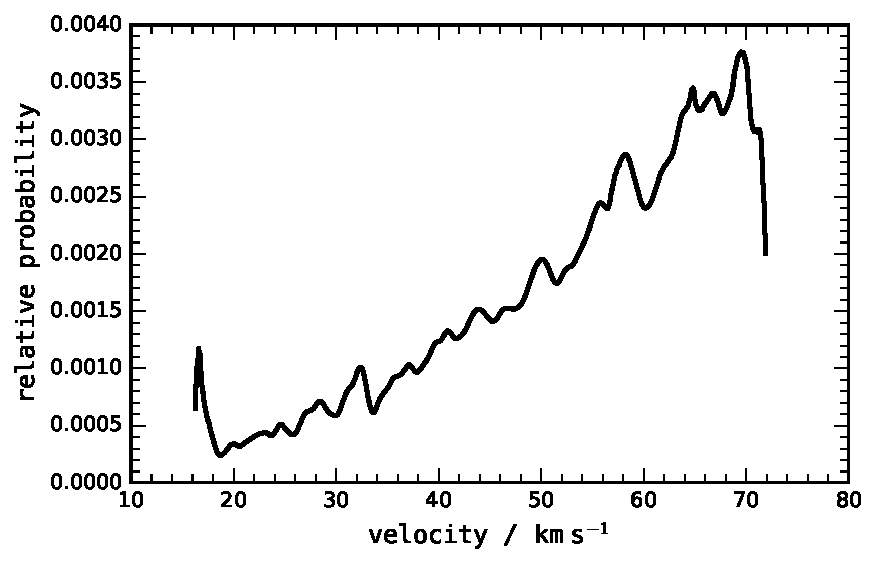
\includegraphics{vel_dist.pdf}
    \caption[Velocity distribution of Earth-impacting cometary meteoroids]{Synthetic impact velocity distribution of LPC meteoroids at the Earth.}
    \label{fig:vel_dis}
\end{figure}

\iffalse
\begin{figure*}[t!]
    \centering
    \begin{subfigure}[t]{0.5\textwidth}
        \centering
        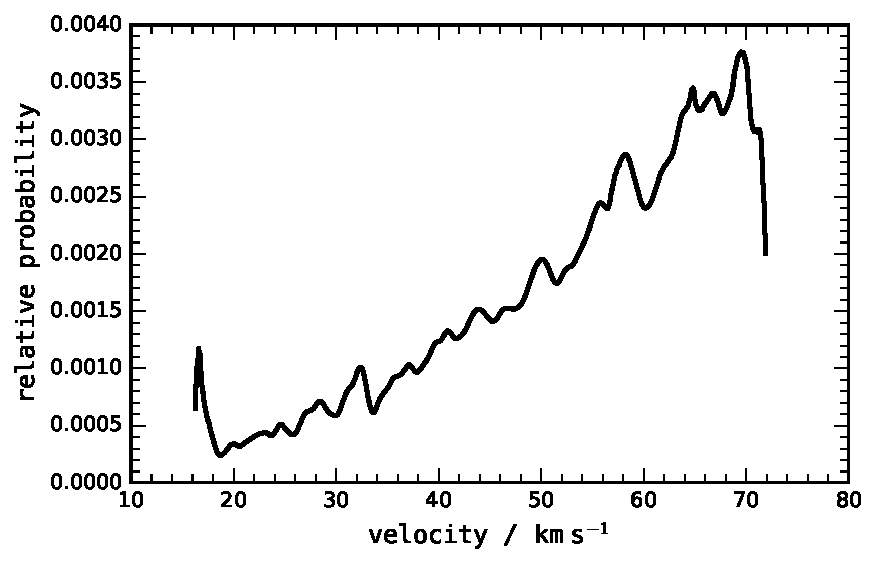
\includegraphics[width=1\linewidth]{vel_dist.pdf}
        \caption{Lorem ipsum}
    \end{subfigure}%
    ~ 
    \begin{subfigure}[t]{0.5\textwidth}
        \centering
        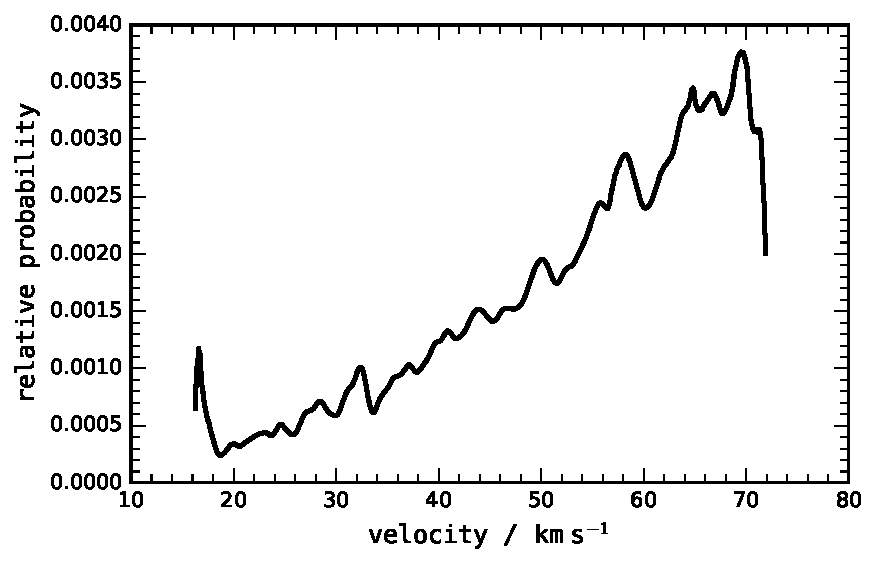
\includegraphics[width=1\linewidth]{vel_dist.pdf}
        \caption{Lorem ipsum, lorem ipsum,Lorem ipsum, lorem ipsum,Lorem ipsum}
    \end{subfigure}
\end{figure*}
\fi

Fig.~\ref{fig:vel_dis} shows the synthetic Earth impact velocity distribution for LPCs. We see that the plot exhibits a peak at both ends of the distribution. These represent the two different extremes of a comet-Earth impact - where a comet is orbiting on the same plane as the Earth and collides on either a prograde or retrograde approach. 

By considering an Earth-impacting comet, with an aphelion very far from the Sun, one can use the escape velocity $v_{esc}$ of the Sun for the comet orbiting on the plane of the ecliptic at 1 AU. Using $v_{esc}=\sqrt{2GM_{\odot}/r}$ where $M_{\odot}$ is the mass of the Sun and $r$ is the distance from the Sun to the comet, the maximum speed for a cometary body impacting the Earth is 42.2 km$\,$s$^{-1}$. This is the maximum velocity for an Earth-approaching comet - otherwise it would not be gravitationally bound to the Solar System. 

By considering a head-on Earth impact as well as an Earth-impact facing the planet behind its direction of travel, the minimum and maximum cometary impact velocities are given by,

\begin{equation}
    (\sqrt{2}-1) \sqrt{ \dfrac{GM_{\odot}}{1 \,\mathrm{AU}} } \leq |v_i| \leq (\sqrt{2}+1) \sqrt{\dfrac{GM_{\odot}}{1 \,\mathrm{AU}}} ~.
\end{equation}
 
These bounds for a cometary meteoroid distribution support the synthetic result shown in Figure.~\ref{fig:vel_dis}. Furthermore, the mean impact velocity is 54 km$\,$s$^{-1}$, in agreement with 53 km$\,$s$^{-1}$ reported by \cite{1988merc.book..274S} for LPC impacts. The calculated distribution was therefore accepted as an appropriate characterisation of impacting comets' velocities for use in the simulation.

%By considering the escape velocity $v_{esc}$ of the Sun for an object orbiting on the plane of the ecliptic at 1 AU, one can use $v_{esc}=\sqrt{2GM_{\odot}/r}$ where $M_{\odot}$ is the mass of the Sun and $r$ is the distance from the Sun to the comet, to calculate the minimum and maximum speeds for a cometary body impacting the Earth. By considering a head-on Earth impact as well as an Earth-impact facing the planet behind its direction of travel - an initial choice for the launch velocity $v$ of each test particle was then selected - such that in the reference frame of the Solar System, the condition $12.4$ km$\,$s$^{-1} \leq |v| \leq 71.9$ km$\,$s$^{-1}$ held true. The absolute minimum and maximum velocity of a cometary meteoroid represent cases where the comet resided on the plane of the ecliptic. This is an unlikely scenario as, for example, LPCs are isotropically distributed. Therefore further selections on velocities were required in order to adequately model the lower expectations for higher-velocity impacts in this range.

%We achieved this by fitting a curve to a meteoroid velocity distribution by \cite{HUNT200434}. This distribution was based on data from the Canadian Meteor Orbit Radar (CMOR) \citep{2014pim3.conf...84W}, which had a large sample size ($>$ 3000) of high velocity meteoroids, making the statistics more reliable for cometary meteoroids.

%The distribution was replicated by fitting two Gaussian distribution functions to the data from \cite{HUNT200434} (See Figure.~\ref{fig:vel_dis}). In order to replicate the distribution, the first Gaussian fit was used for the range 17 km$\,$s$^{-1}$ to 48 km$\,$s$^{-1}$ and the second Gaussian fit was used in the range 48 km$\,$s$^{-1}$ to 72 km$\,$s$^{-1}$.

%The requirement for two curves needing to be fit to the distribution was assumed to be indicative of asteroid and cometary meteoroids. Due to the difficulties in extracting the cometary velocity distribution alone - the velocity distribution representative of all asteroidal and cometary meteoroids was chosen. A filtering mechanism was then employed at the conclusion of the simulation based on dynamical characteristics, in order to extract the cometary population alone (detailed in \S~\ref{chap:results}). For each particle, the velocity of the Earth-Moon system was summed onto a velocity sampled from this replicated distribution.

For each test particle in the simulation, an initial choice of velocity was randomly selected from the generated distribution. Additional final considerations were then applied to the selected velocities. Due to the nature of the random sampling of velocities and positions it was, for example, entirely possibly for a test particle to be assigned a position on the surface of the Earth-Moon system with a velocity vector that caused it to fall towards the Earth upon a reverse-step integration. As this is not the intended behaviour for this simulation of Earth-impacting comets, additional checks were required. If the velocity vector was directed inside the Earth-Moon system, the test particle's location and velocity was reselected. Additionally, if the magnitude of the velocity vector (when summed to the velocity of the Earth-Moon system) exceeded 72 km$\,$s$^{-1}$, the velocity vector was rejected and a new one selected.

\clearpage
\subsection{Launching Routine}

In order to replicate impactors arriving at Earth at different time periods, the population of test particles were gradually released over a time period of 12 yrs. The time period for launches was determined by a random generator using a normal distribution.  The reason for this decision was because Jupiter plays one of the most important roles in influencing the orbits of small bodies in the Solar System - and releasing the test particles over a time period similar to the orbital period of Jupiter was an important decision to help replicate the various different gravitational interactions small bodies have with Jupiter at different points in its orbit.

The Solar System is chaotic, with a Lyapunov timescale of $\sim 5$ Myr \citep{1996CeMDA..64..115L}. A time period of 10 Myr was chosen to be the length of the simulation, in order to fully capture a period of Solar System stability. The integration routine ran with a reverse time step of 6 days, with data snapshots taken every 500 years. At each snapshot the orbital parameters of each simulated body were recorded and written to a .hdf5 file for later analysis. The length of our integration was chosen such that there was not an unnecessarily large expenditure of computing resources, while physically meaningful results were still produced.

\begin{figure}[t!]
    \centering
    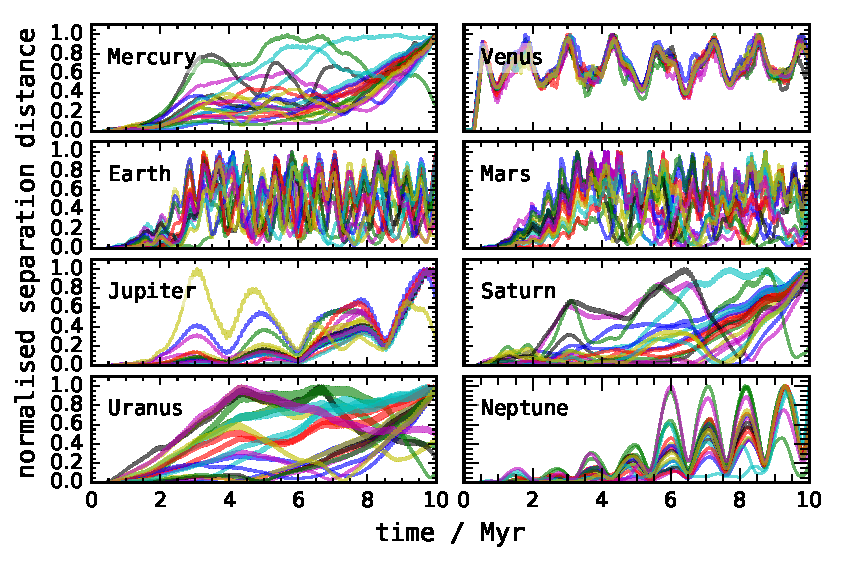
\includegraphics{info_loss.pdf}
    \caption[Parallel Simulations]{(Heavily smoothed) normalised separation distances for each planet in each simulation, from the positions of the planet in the first simulation.}
    \label{fig:info_loss}
\end{figure}

\clearpage
\subsection{Numerical Accuracy}
\label{sec:accuracy}

The nature of the simulated test particles meant that they only gravitationally interacted with the planets, and not with each other. Additionally, the computation time for an N-body simulation scales with the amount of particles. Therefore, in the interests of computational and storage constraints, the simulation was executed as a set of 21 parallel simulations, considering the ejection of $\sim2\times10^{4}$ particles in total.

Chaotic systems such as the Solar System are extraordinarily sensitive to initial conditions. Therefore, position differences on the order of metres between two simulations can lead to completely different dynamical system configurations after $\sim5$ Myr. A lack of robustness between results does not necessarily mean an N-body integration does not accurately represent reality. However, it does mean that for the scope of this investigation we explore the various dynamical pathways explored by comets integrated backwards in time, and are not concerned with retracing the comets' paths continuously back to their source reservoirs.

Because of rounding errors incurred due to floating point operations in the \texttt{MERCURIUS} integrator, the evolution of planets across all the simulations did not perform identically. Fig.~\ref{fig:info_loss} examines the discrepancies in the positions of the planets across all the simulations. The maximum absolute separations for each planet ranged from a minimum of $4.5\times10^{-5}$ AU (Mercury) to a maximum of 0.14 AU (Jupiter). This suggests that the information losses involved are due to a difference in orbital phase, and not due to substantial differences in position.

A large divergence is observed at the 2.5 Myr for most planets, with the notable exception of Venus. One possible explanation for this behaviour is that this sudden growth is due to a resonant interaction with the giant planets.

The divergences across the simulations does not compromise the output data when analysed as a whole. Each simulation represents a unique Solar System environment, where the the changes in comet orbits are consistently governed by the same dynamics throughout. 

Across all the simulations used in this investigation, the mean relative energy error was maintained at $10^{-7}$. Due to the choice of timestep, the energy error throughout the integrations were characterised by an unbiased random walk caused by round-off errors in floating-point calculations. There were some instances of significant energy jumps (still of order $10^{-7}$). This was assumed to be due to very close encounters with major planets that were not properly resolved.

\iffalse
\begin{figure}[t!]
    \centering
    \includegraphics{error.pdf}
    \caption[]{}
    \label{fig:error}
\end{figure}
\fi

\iffalse
\section{Simulating Earth observations of an impending comet impact}

\begin{equation}
    m = H + 5\log(r_{hel}r_{geo}) - 2.5\log(\phi(\theta))~.
\end{equation}
\fi



\iffalse

\subsection{Generating a synthetic population of hazardous long-period comets}

We first generate a synthetic population of hazardous long-period comets, by creating a population of comets subject the following orbital constraints on semi-major axis $a$, inclination $i$ and perihelion distance $r_p$,

\begin{equation}
    \begin{gathered}
        2000 \text{ AU} \leq a \leq 100,000 \text{ AU}~,\\
        0^{\circ} \leq i \leq 180^{\circ}~\\\
        6 R_\odot \leq r_p \leq 1 \text{ AU}~.
    \end{gathered}
\end{equation}

The resulting orbits were then modified further so that they become Earth-impacting. This is carried out by first finding a value of $\theta$ such that $f(\theta)$ is minimised where,

\begin{equation}
    f(\theta) = | \, r_{\Earth} - ||\vec{r}(M = \theta, \omega = 0, a, e, i, \Omega)|| \, | ~,
\end{equation}

and,

\begin{equation}
   r_{\Earth} = ||\vec{r}(M_{\Earth}=\Omega, \omega_{\Earth}, a_{\Earth}, e_{\Earth}, i_{\Earth}, \Omega_{\Earth})||~,
\end{equation}

where $r$ is the distance between the object and the Sun.

A value for $\phi$ is then found such that $f(\phi)$ is minimised where,

\begin{equation}
    g(\phi) = | \, \vec{r}(M = \theta, \omega = \phi, a, e, i, \Omega) \cdot \vec{z} \, | ~,
\end{equation}

where $\vec{z}$ is the Earth's orbital normal vector.

A random lead time $t_l$ is then found, subject to constraints. The comet's and Earth mean anomalies are set to $M = \theta^{\prime}$ and $M_{\Earth} = \theta^{\prime}_{\Earth}$ respectively,

\begin{equation}
    \begin{split}
        \theta^{\prime}_{\Earth} &= \Omega - \dfrac{t_l \sqrt{GM_\odot}}{2\pi {a_{\Earth}}^{3/2}}~, \\
        \theta^{\prime} &= \theta - \dfrac{t_l \sqrt{GM_\odot}}{2\pi {a_{a}}^{3/2}}~.
    \end{split}
\end{equation}

where $M_\odot$ is the mass of the Sun.

\fi
  \chapter{Simulation Results \& Discussion}
\label{chap:results}

We perform a large simulation that considers the scattering of small bodies through the Solar System and produce a population of comets that impact Earth. From this we hope to understand how comets, in particular those from the Oort cloud, are injected into the planetary region and onto Earth-crossing orbits. By analysing a range of orbital behaviours exhibited by these comets, we hope to discover interesting and potentially exploitable behaviour in the sky-plane distribution in the months leading up to a comet impact with our planet.

Throughout this analysis we describe `particles' in simulation, with the direction of time going backwards from the point of Earth impact at $t=0$ Myr. Where there is reference of comets, the direction of time is reversed, from a comet's early dynamical lifetime towards an impending Earth impact.

\section{Migration from Earth-crossing orbits}

Reflective of the extreme velocities of LPCs, the majority of particles in the simulation ($\sim60$\%) were immediately ejected onto hyperbolic orbits, and managed to leave the Solar System without becoming captured due to any planetary perturbations. As detailed in \S~\ref{method:evol}, our primary focus in this analysis concerns dynamically evolved comets and their migration through the Solar System.

Fig.~\ref{fig:migration} shows particles that were initially gravitationally bound to the Solar System and that remain bound throughout the length of the simulation. At $t=0$ Myr, all the particles are within the region bounded by the left and right dashed lines, denoting the Earth's aphelion $r_{ap}$ and perihelion $r_{per}$. The left and right dashed lines are described using the equations $r_{ap} = (1+e)a$ and $r_{per} = (1-e)a$. This region is known as Earth's loss cone, and is discussed in more detail in \S~\ref{sec:loss_cone}. 

A common dynamical pathway for many particles in the early stages of the simulation involves particles migrating out of the loss cone because of increases to their semi-major axis, causing them to typically adopt orbits characteristic of NEOs. The majority of these particles then eventually depart the NEO regions after some time and normally adopt orbits around the giant planets, or are ejected. After $\sim2$ Myr the distribution of particles remains roughly constant throughout the Solar System.

Particles with low semi-major axes populate the near-Earth region with aphelia close to that of Earth's. These particles tend to migrate away from Earth with decreasing $a$ up to a point, where they either are rapidly scattered towards regions of the outer Solar System or are returned to orbits close to the Earth-Moon system. It would be reasonable to assume that particles ejected in this manner, that also have low inclination orbits, are likely to collide with the Earth-Moon system again at some point after ejection. As planetary collisions have been neglected in this simulation, it is presumed that the prevalence of such comets remaining close to this region of $a$-$e$-$i$ space in Fig.~\ref{fig:migration} for the majority of their dynamical lifetimes are not realistic.

Particles with eccentricities very close to 1 (as seen located near the horizontal cut-off at the top of the plots) require little energy to become unbound. As expected, these highly eccentric particles rapidly depopulate this area of $a$-$e$-$i$ space within the first few thousand years.

A few particles that are initially ejected onto extreme orbits (very high inclinations $i > 150^\degree$ and high eccentricities $e>0.5$), which have significantly low values of $T_J$ in comparison to the rest of the cometary ejecta, are seen to remain largely undisturbed by planetary interactions throughout the course of the simulation.  Highly inclined orbits minimise time spent close to the ecliptic, reducing the chance of an interaction. These particle retain $a \approx 1$ throughout the 10 Myr length of the simulation.

If one assumes that a LPC has an equal probability to become gravitationally scattered on to any of the available orbital parameters, it is likely that the comet is scattered onto a value of $T_J$ close to its original value (due to the quasi-constant nature discussed in \S~\ref{sec:taxonomy}). Therefore, the probability of LPCs evolving from the Oort Cloud onto extreme orbits with $a$ on the order of Earth's is anticipated to be low. Such particles are expected to have small orbital periods, and remain near Earth for substantially long periods of time - for many orders of magnitude of time longer than their physical lifetimes may permit in this inner Solar System environment.

%FINISH THIS, THEN LOSS CONE (AND PROPER PLOT). Finish discussion with leading onto decision tree. Work out bad comets.
%add a table for something

%finish loss cone and resonance
%find bad comets for plot and mitigation

\begin{figure}[t!]
    \centering
    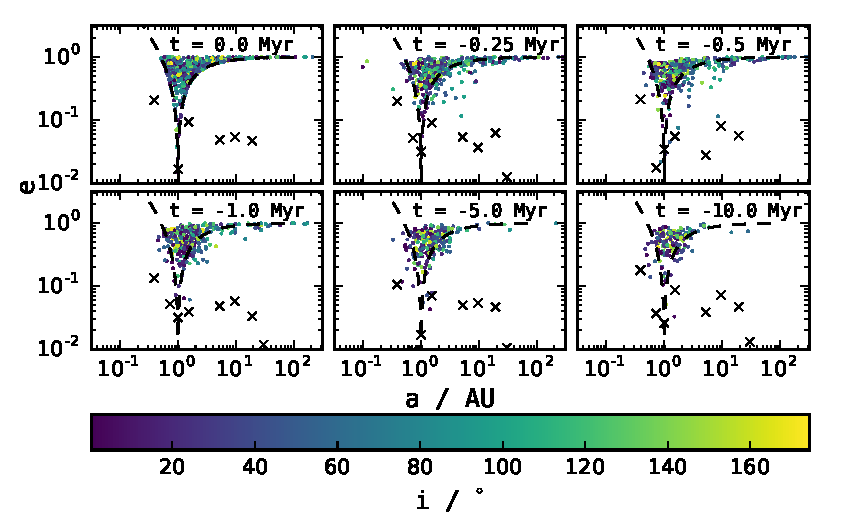
\includegraphics{ae_migration.pdf}
    \caption[Particle Migration]{Gravitationally bound particles in the simulation at various snapshots in time. The boundaries of the Earth's loss cone are marked with dashed lines. The first 8 planets of the Solar System are plotted as black crosses.}
    \label{fig:migration}
\end{figure}

\section{Dynamical lifetimes}

\subsection{Exiting the Solar System}

For each cometary particle in the simulation we calculated the dynamical lifetimes by determining the length of time taken for gravitational perturbations to render the particle's orbit unbound. The median dynamical lifetime was found to be $4.1\times10^5$ yrs. This is of the same order of magnitude as $6\times10^5$ yrs for LPCs reported by \cite{1979IAUS...81..277W}, with a smaller value perhaps indicative of the reduced likelihood for LPCs to reach further into the Solar System and encounter Earth.

The initial population of test particles was observed to decay approximately exponentially for the first 2 Myr of the simulation, before declining at an almost constant rate at times greater than the typical dynamical lifetime. The constant decline in the cometary population at later times is unexpected, as one would assume that the probability of gravitational perturbations by the planets remains unchanged. With a dwindling population of bound particles in the simulation as time progresses, one would expect the leaving rate to continuously decline and the numbers of surviving particles remaining in the simulation to become governed by some form of power law behaviour \citep{1996ASPC..107..233D}. 

We instead find a long-lasting population of comets with dynamical lifetimes exceeding the 10 Myr of the simulation. A subset of this long-lasting population had $a < 2$ AU, and were assumed to be unrealistic due to physical losses due to small heliocentric distances over a long period of time. The remaining objects tended to migrate from the very far reaches of the Solar System ($>$ 600 AU) prior to an impact with Earth. and were found to effectively have become stored in large, stable orbits for periods of time much longer than 10 Myr. 

\subsection{Prograde vs Retrograde orbits}

While the overwhelming majority of asteroids have prograde orbits - many comets (eg. 1P/Halley) are known to have a retrograde orbits. Around 50\% of comets arriving from the Oort Cloud are retrograde.

The energy kicks delivered by the prograde planets upon passing comets should be smaller on average for comets on retrograde orbits than prograde orbits. The result of this is that retrograde comets should have dynamical lifetimes three times longer on average. In the absence of physical decay mechanisms, this means the ratio of retrograde to prograde comets should be 3:1.% This behaviour should manifest itself through the appearance of various transfer pathways for simulated test parts, depending on whether they are prograde or retrograde. 

The initially bound retrograde comets in the simulation had a median dynamical lifetime of $6.4\times10^5$ yrs compared to a median dynamical lifetime of $1.8\times10^5$ yrs for initially bound prograde comets, meaning that the ratio of retrograde to prograde comets should be roughly 3:1 for our simulation. This indicated that prograde comets are more favourably scattered, and that a greater number of much more energetic, retrograde comets reach Earth's orbit.

%Figure.~@@@@@ PUT STUFF HERE

\section{Random Walks in energy space}

\begin{figure}[t!]
    \centering
    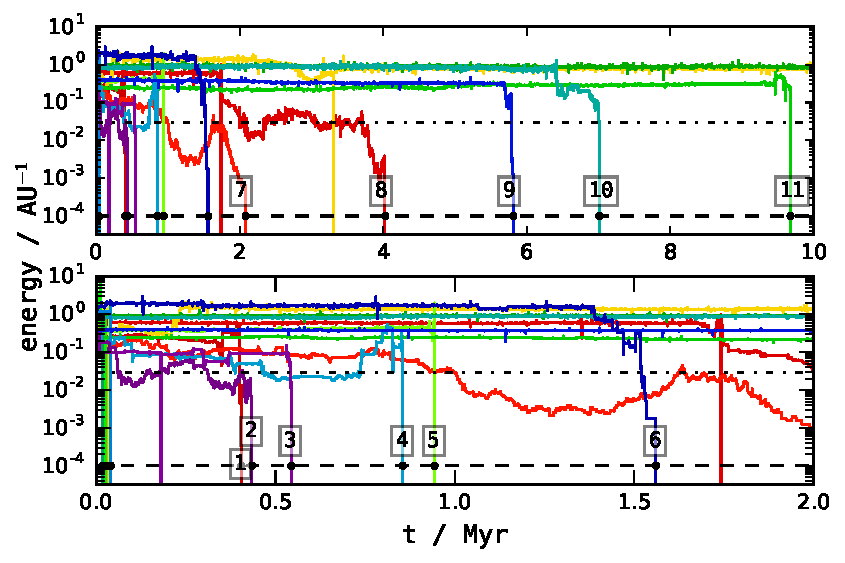
\includegraphics{figures/ae_timeplot.pdf}
    \caption[Random walks in energy space]{Temporal evolution of comet orbital energies. Top: Energy paths of randomly selected comets between $0<t<10$ Myr, shown in different colours. Bottom: Same comets evaluated between $0<t<2$ Myr. Short period comets with P $<$ 200 yr are found above dash-dot black line at 0.0292 AU$^{-1}$.  Comets beginning their dynamical evolution through the Solar System are found below the dashed black line at $10^{-4}$ AU$^{-1}$. Black dots mark the transitions of comets coming from dynamically new regimes for the first time, between the times 0.05-10 Myr, and are labelled for reference.}
    \label{fig:timeplot}
\end{figure}

%http://adsabs.harvard.edu/full/1980A%26A....85...77Y diffusion eq
An analysis of the scattering mechanisms of dynamically new LPCs that are just beginning their evolution through the Solar System is an important first step in considering how comets  either i) migrate towards more tightly bound orbits and deeper into the Sun's gravitational potential towards Earth, or ii) are scattered onto unbound orbits and quickly leave the Solar System.

The dynamical evolution of LPCs through successive interactions with planets in the Solar System is often described as a stochastic process, in which a comet interacts every successive perihelion passage with a planetary configuration unique to the previous interaction. As LPC aphelia lies well beyond the reach of the Solar System, the planets' gravitational influence dominates at perihelion passage, and can be approximated with an instantaneous kick in orbital energy, where $x = (1/a)$ is the binding orbital energy of an object on a Keplerian orbit. These kicks are symmetrically distributed about zero, and are uncorrelated as long as the comet's orbital period remains much larger to that of the planets. 

The energy of highly eccentric comets evolves on much shorter time scales than orbital elements such as perihelion $q$, inclination $i$, longitude of ascending node $\Omega$, argument of perihelion $\omega$. Therefore one can, as a first-order approximation, conceive the orbital evolution of LPCs as a one dimensional random walk behaviour in energy space. This is distinct from other more dynamically evolved objects in the Solar System which exhibit different dynamics, (eg. those with resonant behaviours). 

This behaviour is exhibited in Fig.~\ref{fig:timeplot} where we can observe the random walk behaviour of LPCs injected into the planetary system. We consider two absorbing walls in energy space; ejection onto an unbound orbit $(x > 0$ AU$^{-1})$ , and transfer to a periodic regime $(x < 0.0292$ AU$^{-1})$ corresponding to $P < 200$ yr (dot-dashed line). Dynamically young comets, probably on their first passage into the Solar System from the Oort Cloud, have energies below $(x < 10^{-4}$ AU$^{-1})$ (dashed line).

While most comets are rapidly injected towards the periodic orbit energies, some comets persist in energy space between the two absorbing walls for considerably lengths of time. We find an excess of paths in Fig.~\ref{fig:timeplot}, notably 6,7 and 8, that correspond to retrograde comets. This demonstrates that retrograde comets evolve much slower in this energy space due to lower probabilities of being caught by the planets. Such lengths of time spent in the outer reaches of the Solar System suggest that retrograde comets have ample time to fade sufficiently, before progressing to dynamically older states in regions in which they can more easily be observed from Earth.

Prior to an impact with Earth, 3, 4, and 8 in in Fig.~\ref{fig:timeplot} can be seen to have entered the region in energy space between $(0.0292 < x < 10^{-4}$ AU$^{-1})$. Such behaviour is believed to be unlikely as the typical energy change of a comet per revolution is of the order $\sim10^{-3}$ AU$^{-1})$. A return to `dynamically newer' states may also be unrealistic once non-gravitational forces are taken into account. The actions of non-gravitational effects may complicate the simple statistical considerations of randomly-walking comets, and provide systematic increases or decreases to the orbital energy of comets. The result of this means that the dynamical evolution of comets is much faster once non-gravitational considerations are met, leading to comets becoming much less sensitive to transitions to and from this dynamically new region of energy space.

Some comets, for example those following the paths 1, 5, 9, 10 and 11, are rapidly injected into the Solar System, spending no more than a few perihelion passes in the space between the two absorbing walls. These comets quickly find themselves in long-lasting, tightly-bound orbits where the systematic gravitational effects of the planetary environment become much more relevant. The oscillatory behaviour of the orbital energy suggests these comets have quickly become trapped in stable orbits governed by mean motion resonances (MMRs) (see \S~\ref{sec:resonance}).

%https://projecteuclid.org/download/pdf_1/euclid.bsmsp/1200512808

\section{Resonance}
\label{sec:resonance}

Although generated with cometary dynamical properties, some particles throughout the simulation behaved strikingly similar to NEAs, which are known to chaotically migrate from the inner Solar System due to the effects of repeated close encounters with terrestrial planets, and the effects of MMRs and secular resonances.

Once becoming ejected from the Earth-Moon system, some particles in the simulation have scattered between the terrestrial planets before eventually entering stable orbits via strong resonances. These resonances are easily detected from the analysis of the temporal evolution of $a$, identifying where there are small-amplitude oscillations around a constant mean value $\langle a \rangle$. 

We study MMRs in particular by studying the mean averages of $a$ in windows of $10^4$ yrs. We identify the locations of $p$:$q$ resonances using $a_{mmr} = a_p (p/q)^{2/3}$ where $a_p$ is a planet's semi-major axis. This reveals a distribution in $\langle a \rangle$ with strong peaks corresponding to resonances up to the 1:21 external MMR with Jupiter. The majority of comets `stuck' in these stable librations are retrograde, which can be understood by the reduced influence of Jupiter on retrograde orbits. 

We also find peaks in $\langle a \rangle$ revealing large Trojan populations of comets stuck in 1:1 capture resonances with Jupiter and Neptune. For all comets stuck in these MMRs, we found that at least 20\% of their dynamical evolution time was spent within $\pm.1$ AU of any of these resonances. We also find comets become captured into Saturn and Uranus crossing orbits, but find themselves ejected quickly, possibly due to an orbital instability introduced by Jupiter.

Throughout a comet's lifetime both random walk and resonant behaviour become important at separate points in time, as well as largely influential for particular classes of comets. In the simulation, the long-term survival of the particles ended up being much greater than predicted by purely diffusive behaviour - a result attributed to the interplay of both these dynamical behaviours.

From Table.~\ref{table:class}, one can see that the particles that migrated from Earth and into the Centaur dynamical class spent an average of $3/4$ of their dynamical lifetimes with this behaviour. From the population of these Centaur particles we find that migration from Earth-crossing orbits is a rapid and chaotic path through the Solar System, rapidly raising their $a$ up to distances comparable to Uranus' in an amount of time equal to the average of 3\% of their dynamical lifetimes. A qualitative analysis of the Centaur particles revealed two distinct groups - one consisting of comets characterised by diffusive behaviour, and  another group of Centaurs dominated by resonant behaviour for almost the entire lengths of their dynamical lifetimes. Particles were likely to leave the Centaur class by evolving to HFCs or JFCs. There was a clear predominance of retrograde orbits for the particles that exited the Centaur class by rapidly moving towards Oort Cloud energies.

The populations with $q < 1.3$ AU of the HFCs and JFCs in the simulation remained of comparable size throughout the length of the integration. HFCs were likely to become gravitationally ejected after migrating into MMRs with Jupiter, in particular the exterior 1:q exterior resonances. JFCs, being more strongly coupled with Jupiter, were more likely to remain bound and migrate outwards to the far reaches of the Solar System.

\begin{table}[t!]
\centering
\caption[Particles classes and their mean dynamical lifetimes]{Classifications of test particles in the simulation and the average \% of the particle's dynamical lifetime spent in that class. Classifications into either a Jupiter Family Comet (JFC), Halley Family Comet (HFC), Centaur, Trans-Neptunian Object (TNO) or Encke-type comet. Class definitions based on the Jovian Tisserand parameter $T_J$, orbital period $P$, perihelion $q$, and semi-major axis $a$.}\vspace{1.5ex}
\label{table:class}
\begin{tabular}{ccc} \toprule \toprule
Taxonomic Class & Classification                                      & Mean \% dynamical time \\ \midrule
JFC             & $2 < T_J < 3$; $P > 20$ yrs & 26.86                  \\
HFC             & $T_J < 2$; $P < 200$ yrs               & 42.60                  \\
Centaur         & $q > 5.2$ AU, $a < 30.1$ AU          & 69.18                  \\
TNOs            & $a > 30.1$ AU                              & 26.13                  \\
Encke-type          & $T_J > 3$; $a < 5.2$ AU             & 70.31                 
\end{tabular}
\vspace{-3ex}
\end{table}

%leave resonances by increase in libration or A torque is applied that is stronger than the resonance can tolerate.
%https://history.nasa.gov/SP-345/ch8.htm
%MAIN BELT COMETS
%ALSO IN 1:1 WITH NEPTUNE


%more from %https://arxiv.org/pdf/1606.05603.pdf

%stable vs unstable resonances capture resonances
%commensurabilit/near commensurability
%BREAKING THE RESONANCE Comets: Nature, Dynamics, Origin, and their Cosmogonical Relevance resonance P85

%Resonance Hopping vs random walk diffusion LOOK AT THIS
%https://eprints.usq.edu.au/28888/1/CentaursJeremy.pdf

%this study supports the idea that Centaurs do represent a threatto Earth.
%Of thetaxonomicalclasses inward from the resonance, the Encke-type cometclass had the highest average occupancy time at 33\%. Of the outward classes,KBO had the highest average occupancy time at 14.9\% of a test particle’s lifetime. 65\% of a sample of Earth crossers were random walkers and 35\%resonancehoppers.Graphs of semi-major axis vs. time for resonance-hopping Centaurs tend to have long horizontal bands, and those of the random-walk Centaurs tend to lack long horizontal bands

\section{The Encke Problem}

Of the taxonomical classes in Table.~\ref{table:class}, the Encke-type comets made up the longest occupancy times at 70\%. The comets were decoupled from Jupiter, with aphelia $Q < 4.2$ AU, with $a$ interior the Jupiter 3:1 MMR and $a < 2.4$ AU. These comets typically find themselves embedded in asteroid populations at low inclinations; these asteroid populations themselves perhaps consisting of extinct cometary nuclei. Object in these orbits constitute a significant fraction of the Earth impact flux.

Of all the Encke-type comets investigated in the simulation, the second most likely dynamical class for such objects to be in during their lifetimes was found to be the HFC class. This reveals the presence of a purely gravitational dynamical pathway (produced by the terrestrial planets) for LPCs to rapidly evolve into Encke-type classes. This is of particular significance, as it suggests that a large population of dormant comet nuclei may exist in NEO populations, masquerading as asteroids and therefore impacting our understanding  of  the  relative  importance  of  asteroids  compared to comets as part of the impact hazard.

The majority of these comets' lifetimes were found to be spent in this Encke-type class, with a median dynamical lifetime of 7.89 Myr. This suggests that like the asteroids which such comets cohabit regions of the Solar System with, the small body populations are unlikely to fluctuate wildly on short-term, human timescales due to the introduction of a comet shower. Additionally, the dynamical lifetimes far exceed the expected estimated amount of time required for a comet to physically age, and become dormant or fragment. This suggests that redoing the simulation with realistic modelling of the physical aging of comets would apply additional constraints on these Encke-type comets -  and allow only anomalously large and long-lived comets to persist into such orbits. Alternatively, it could also mean that a population of multi-kilometre, long-lived and extreme low albedo comets could exist in the NEO environment, unbeknownst to current Earth object surveys.

%encke Type comet impacts
%comet fading to dormant JFCs
%https://pdfs.semanticscholar.org/db45/cffd0d3ef903498c5e80b2358d3f632717a7.pdf
%we define ‘Encke-like’to mean those objects decoupled from  Jupiter (Q<4.2AU)with semi-major axes interior to Jupiter’s 3:1 mean motion reso-nance (a<2.4 AU). 

%size and shapes of cometary nuclei http://adsabs.harvard.edu/abs/2004come.book..223L
%http://www.astro.uwo.ca/~wiegert/papers/2006Icarus.182.161.pdf
%\section{Fragmentation}

%clustering of aphelion directions
%exotic particles
%random walk and resonance hopping
%\cite{1997astro.ph..5153W}

\section{Jupiter-Saturn Barrier}
\label{js-barrier}
%https://arxiv.org/pdf/0911.4381.pdf
As infalling comets proceed on a random walk in $1/a$, the planetary energy kick imparted by the giant planets in the 10-15 AU range is typically much larger than the gravitational binding energy of inbound Oort Cloud comets that are only tenuously bound to the Solar System. Therefore, the expected perihelion drift of LPCs falling into the inner Solar System is expected to halt in the $\sim$10-15 AU domain where comets become rapidly unbound from the Solar System, or perturbed onto low $a$ orbits before then eventually becoming ejected. This mechanism, known as the Jupiter-Saturn barrier, is hugely influential in influencing cometary motion, responsible for significantly reducing the impactor population reaching Earth.

Analysis of all the Earth impactors that pass through the Jupiter-Saturn zone revealed that a smooth drift in $q$ followed by a rapid inflation in $a$ that occurs around the 15 AU point - as LPCs move inwards toward regimes of more rapid orbital evolution. This effect obscures the Oort Cloud origin of such comets, but more importantly allows them to prevail against the `leaky' Jupiter-Saturn barrier. 

Retrograde comets are again observed to be more successful in penetrating the barrier, due to weaker planetary perturbations.

Objects with $a\sim 3\times10^4$ were particularly efficient in circumventing ejection by the Jupiter-Saturn barrier - partly because these objects would require less energy kicks by the planets to reach perihelion distances beyond the gas giants. No particles in the simulation were found to move through the Jupiter-Saturn barrier with diffusive behaviour characterised by a nearly constant $a$ - the orbital evolution of the particles was instead markedly dominated by rapid changes in $a$. When analysing the distribution of $\langle q \rangle$, the moving average of perihelia in windows of $10^2$ yrs, no particles were found to have $10 < \langle q \rangle < 20$ AU.

Many particles in the simulation that persisted safely throughout the inner Solar System then became ejected upon reaching the Jupiter-Saturn zone in their backwards integrations. This suggests that Jupiter and Saturn provide a very efficient barrier effect that places large constraints on the various dynamical pathways towards the inner Solar System through the 10-15 AU range. These ejected particles represent comets that may not have realistically overcome the Jupiter-Saturn barrier when evolving forwards in time.

The larger the value of $a$, the less of a perturbation comets encounter from the Jupiter-Saturn barrier. Therefore, inbound LPCs that have been thrown out of the Oort Cloud by a strong perturber such as a close passing star are more likely to overcome the barrier as opposed to comets with smaller $a$, due to perhaps being perturbed by the galactic tide. This raises the prospect of an exceptionally large comet shower overcoming the barrier over short timescales. The ensemble of orbits in a comet shower passing the Jupiter-Saturn zone all at once would manifest itself as the rapid population of a somewhat sparse region of velocity space known as the loss cone (detailed in \S~\ref{sec:loss_cone}). %TALK ABOUT COMETS SHOWERS and leads into jupiter/loss cone segue
%Objects in a comet shower from the Oort Cloud are likely to have velocity vectors close to the solar direction, part of the configuration of a comet's orbit that makes it liable to removal through a range of dynamical and physical processes due to interaction with the Sun.
%p7 https://arxiv.org/pdf/1801.01474.pdf

\section{Loss Cone Dynamics}
\label{sec:loss_cone}

\begin{figure}[t!]
    \centering
    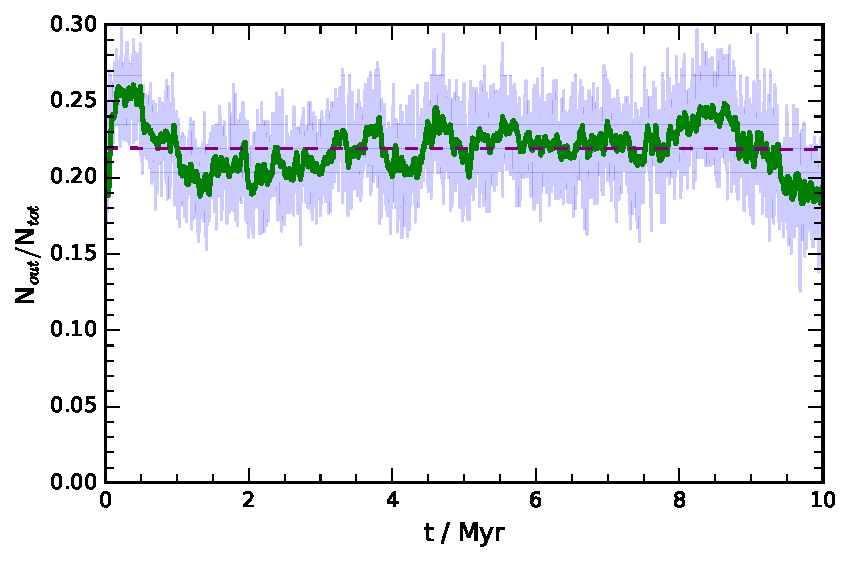
\includegraphics{figures/exotic_ratio.pdf}
    \caption[]{}
    \label{fig:exotic}
\end{figure}

A population of comets falling inwards from the Oort Cloud will have randomly oriented orbits where all approach directions are possible. Comets falling very close the solar direction are likely to get boiled away and disintegrated by the Sun, or alternatively may swing by one of the planets and pick up enough extra speed from the encounter to carry it right out of the solar system. In either case, these particular comets are lost from the Solar System. Consequently, there is an region of energy-angular momentum space around the solar direction that is expected to be particularly devoid of LPCs. This is known as the Sun's loss cone, and was shown by \cite{1981AJ.....86.1730H} to be effective in shielding the Earth from showers of comets.

This loss cone concept is similar to considerations of stars or stellar remnants accreting into black holes \citep{0264-9381-30-24-244005}. The formulation of a loss cone can be extended to other bodies of the Solar System, and is described as a set of orbits of sufficiently low angular momenta such that they intersect a certain body, or pass within some distance of its centre. %The critical angular momentum $J_{lc}$ of a loss cone for a periapsis of the central body $q$ is,

%\begin{equation}
%    J_{lc}^2 = GM_\odot q(1+e)~.
%\end{equation}

%Comets with $J < J_{lc}$ fall within the loss cone and are assumed to become removed over some timescale corresponding to the loss cone's central body.

External perturbations on the Oort Cloud, eg. passing stars, can significantly change the angular momenta of comets and send them into the Sun's loss cone. The Jupiter-Saturn barrier (detailed in \S~\ref{js-barrier}) is unable to provide sufficient orbital angular momenta to such comets for them to leave the loss cone. A loss cone comet can only leave the region by two means; through either hyperbolic ejection, or the destruction of the comet due to breakup near the Sun or a planetary impact. This means that if there is the occurrence of an exceptionally strong shower of Oort Cloud comets, such an event can manifest itself as a rapid filling of the Sun's loss cone, and can therefore be a method of identifying an impending LPC threat to Earth.

In this investigation, we simulate a huge number of comets reaching Earth within an 11.8 year period. Comets capable of an impact with Earth have heliocentric loss cone orbits - which means that the simulation is in effect - an unrealistically very extreme example of a comet shower filling the Sun's loss cone. In addition, we are not concerned in retracing these comets back to an Oort Cloud environment (for reasons detailed in \S~\ref{sec:accuracy}). For these reasons, we neglect analysis of the filling of the Sun's loss cone and focus on smaller regions of angular-momenta space within it, namely the Earth's and other planet's loss cones.
%spend time considering earth loss cone for this sim - we cant really do sun loss cone as we're doing a comet shower anyway
%reference mpc data and talk about how phas are almost all in loss cone of earth

Fig.~\ref{fig:exotic}

\section{Worst-case scenarios}

\begin{figure}[t!]
    \centering
    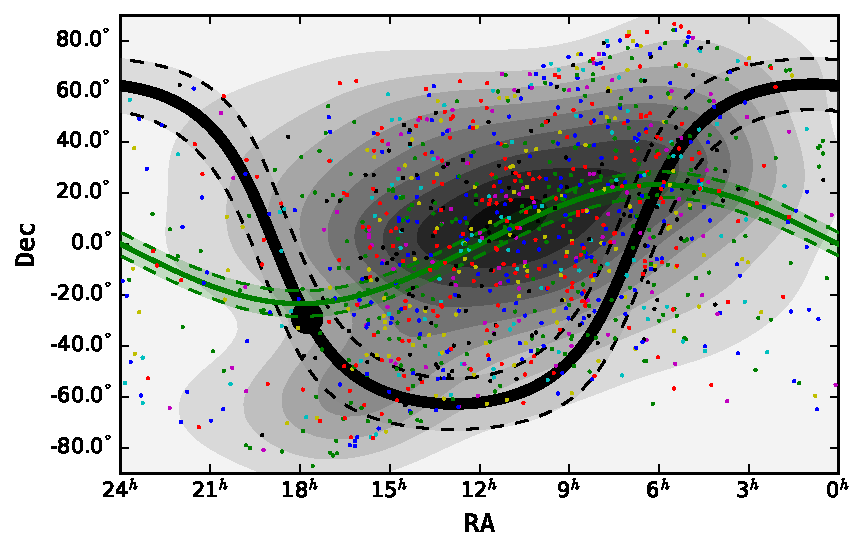
\includegraphics{radiants.pdf}
    \caption[Distribution of apparent radiants]{Distribution of apparent radiants. Geocentric equatorial coordinates plotted for various comet threats. Green line and boundaries represent the plane of the ecliptic $\pm5^\degree$, black line and boundaries represent the galactic plane $\pm10^\degree$. The galactic centre is plotted as black circle. A 2D kernel density estimate is shown.}
    \label{fig:loss_cone}
\end{figure}

% "In principle," he adds, "one would expect those positions to be evenly distributed in the sky, particularly if these objects come from the Oort cloud. However, what we find is very different-a statistically significant accumulation of radiants. The pronounced over-density appears projected in the direction of the constellation of Gemini, which fits the close encounter with Scholz's star.


%prograde vs retrograde plot
%https://onlinelibrary.wiley.com/doi/pdf/10.1111/maps.12080 make fig5
%radiant distribution plot for good lasting comets geocentric equatorial
%lead time calculations
%decision tree of loss cone direct entry time, choose features that match mpc



%dormant comets
%http://adsabs.harvard.edu/full/2004MNRAS.355..191N
%https://academic.oup.com/mnras/article/462/4/3511/2589444





\iffalse

%We operationally define τ stream as the time taken for the median D-parameter of any two test meteoroids to grow beyond a given threshold. The D-parameter was originally introduced by Southworth & Hawkins (1963) for meteor shower identification; it is essentially a measure of the similarity between a pair of orbits denoted as A and B:

\begin{equation}
\begin{split}
    D_{A,B}^2 = (q_B - q_A)^2 + (e_B - e_A)^2 + \left(2\sin{\dfrac{I}{2}}\right)^2
    \\ + \left[(e_A + e_B)\sin{\dfrac{\Pi}{2}}\right]^2 ~,
\end{split}
\end{equation}

where,

\begin{equation}
\begin{split}
    I = \arccos[{\cos{i_A}\cos{i_B}+\sin{i_A}\sin{i_B}\cos{\Omega_A-\Omega_B}}]~,\\
    \Pi = \omega_A - \omega_B + 2\arcsin{\left(\cos{\dfrac{i_A + i_B}{2}\sin{\dfrac{\Omega_A - \Omega_B}{2}\sec{\dfrac{I}{2}}}}{}\right)}~.
\end{split}
\end{equation}

\fi
  \chapter{Conclusion}
\label{chap:conclusion}

We have performed a large scale N-body simulation of cometary dynamics in the Solar System, in an effort to understand the nature of the transport mechanisms that bring impacting comets to Earth. By examining cometary material being continuously scattered through the Solar System, we report dynamical lifetimes in line with previous investigations. 

We discover that impacting comets chart vibrant dynamical pathways towards Earth, with behaviours dominated by resonances, diffusion, and chaos. Such behaviours largely define particular dynamical classes of objects, such as the Centaurs travelling rapid and chaotic routes towards the inner planetary environment. We consider the existence of Encke-type comets masquerading as asteroids in the NEO environment. In the absence of physical decay laws in our simulation model we conclude that such comets are not liable to large fluctuations from comet showers, and that if such a population does exist it may consist of extreme low albedo, long-lived objects that have not yet been detected from Earth.

Throughout our analysis we find that retrograde comets display a propensity to persist and be scattered less in the planetary environment. From this we conclude that dangerous retrograde comets may be more likely to reach Earth, but at the expense of more physical ageing due to a slower orbital evolution.

We conclude that the effects of the giant planets act as a significant protection against comets reaching Earth, with objects of large semi-major axes being particularly efficient at circumventing the barrier effect. This has implications for the prospect of very large comet showers circumventing the barrier and reaching into the NEO environment on short timescales. We find that analysis of planetary loss cones can be a useful tool in differentiating rapidly evolving showers of comets with short warning times from objects of a more asteroidal dynamical nature.

By exploring the use of a decision tree predictive model, we provide an interpretable framework that can be used to identify hazardous cometary material. From the model results we find that while large orbital period and isotropic inclinations make LPCs rare and inefficient Earth impactors, comets destined for a collision with our planet may well already exist in our Solar System. Such a conclusion is based purely on dynamical grounds - and future work involving more explicit modelling of cometary physical processes is encouraged in order to assess any additional constraints that these may introduce.

Our understanding of the geological history of our planet in the context of impact hypotheses is at an early stage, and only more work will reveal whether more exceptionally devastating impacts than we may realise have occurred in the past.

We finish by saying that current planetary defence policy may be fallaciously assuming that comet impacts represent a practically negligible impact hazard, whereas simulations suggest that such an event may be more accurately described as one of a more unknown probability. NEO surveys are currently concentrating on perceiving slowly evolving threats based on what we can observe, and despite considerable advances in the last few years, do not merit the present complete lack of awareness when it comes to considering the fact that comets can also reach our planet, and with terrible consequences.


  \backmatter
  \small %\footnotesize

\addcontentsline{toc}{chapter}{Bibliography}

\bibliographystyle{aasjournal-hyperref}
\bibliography{references}


  \markboth{}{}
  
  \appendix

\renewcommand{\thefigure}{A.\arabic{figure}}
\setcounter{figure}{0}
\renewcommand{\thetable}{A.\arabic{table}}
\setcounter{table}{0}
\renewcommand{\theequation}{A.\arabic{equation}}
\setcounter{equation}{0}

\chapter{Appendix}
\section*{}

\begin{figure}[h!]
    \centering
    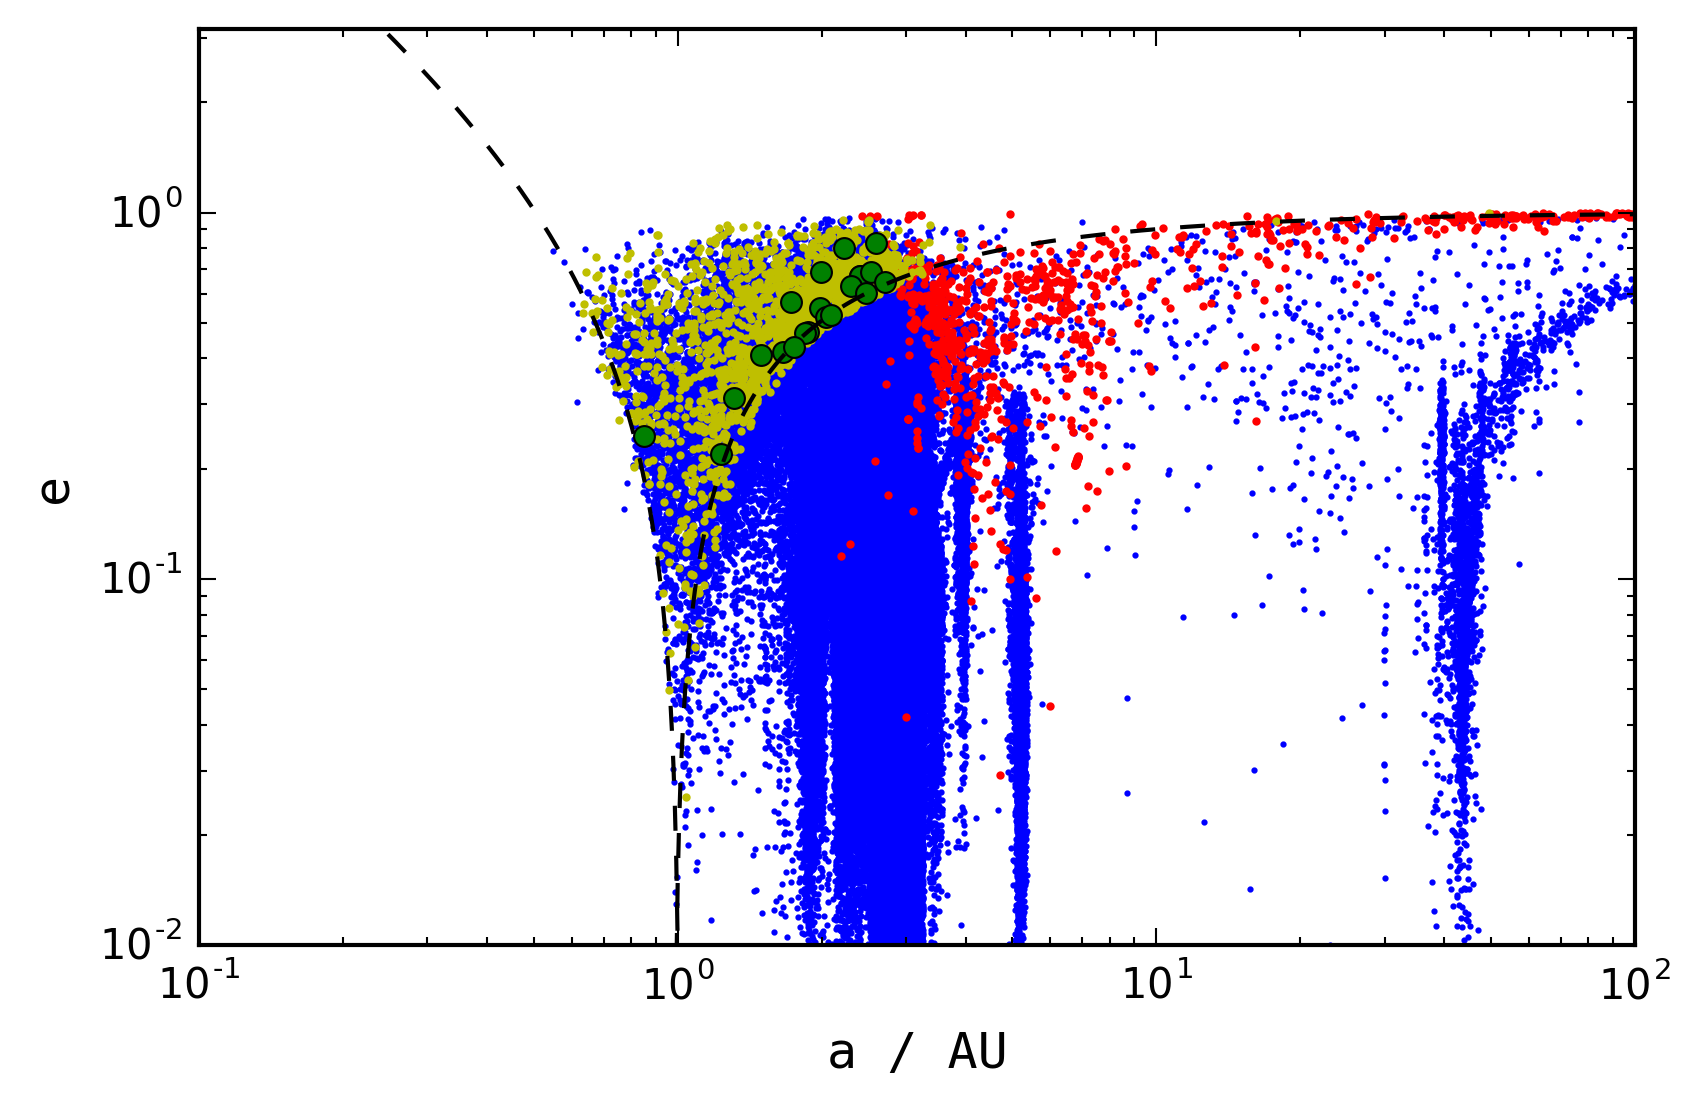
\includegraphics{losscone.png}
    \caption[Catalogued asteroids and comets in Earth's loss cone]{Semi-major axes vs eccentricities of observed asteroids (blue), comets (red) and potentially hazardous asteroids (yellow). Data sourced from the IAU MPC. Meteorites with pre-impact orbits determined by \cite{doi:10.1093/mnras/stv378} are plotted as green circles. The Earth aphelion and perihelion are plotted as dashed lines.}
    \label{fig:loss_cone}
\end{figure}

\begin{figure}[h!]
    \centering
    \includegraphics{figures/error.pdf}
    \caption[Simulation error]{Relative energy error over time. Black line shows the moving average of all the simulation runs.}
    \label{fig:error}
\end{figure}

%\section{Worst-case scenarios}

\begin{figure}[h!]
    \centering
    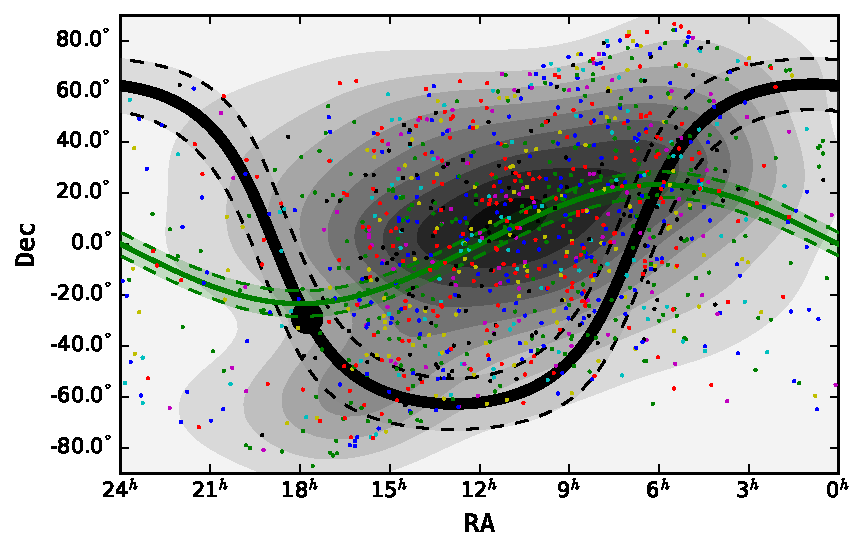
\includegraphics{radiants.pdf}
    \caption[Distribution of apparent radiants]{Distribution of apparent radiants for comets at the point of impact. Geocentric equatorial coordinates (J200) plotted for various comet threats. Comets that spent the majority of the simulation length in the JFC class are marked as triangles. Plus markers for HFCs, circles for centaurs, squares for TNOs and diamonds for Encke-type comets. Different marker colours denote separate simulation runs. Green line and boundaries represent the plane of the ecliptic $\pm5^\degree$, black line and boundaries represent the galactic plane $\pm10^\degree$. The galactic centre is plotted as a black circle. A 2D kernel density estimate is shown.}
    \label{fig:radiants}
\end{figure}

\begin{figure}[h!]
    \centering
    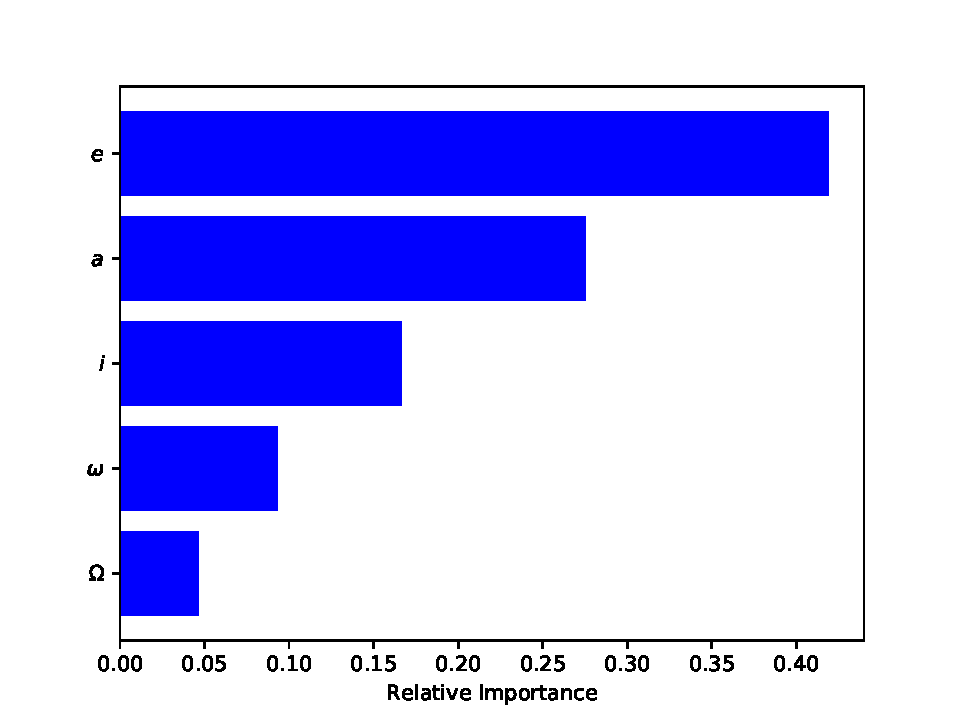
\includegraphics[width=\textwidth]{gini.pdf}
    \caption[Relative importance of orbital characteristics in learning algorithm]{Relative importance of each feature used for classification in the random forest learning algorithm. Gini importance calculated by examining the total reduction of $I_G$ due to a particular feature across all our decision trees.}
    \label{fig:gini}
\end{figure}


\begin{sidewaystable}[h!]
\caption[Initial conditions]{Initial conditions of the solar system as of 01-12-2017 12:00 UTC. Data sourced from NASA JPL Horizons database.}\vspace{3ex}
\label{table:init_con}
\begin{tabular}{llllllll} \toprule \toprule
\multicolumn{1}{c}{Object} & \multicolumn{1}{c}{Mass / $M_{\odot}$} & \multicolumn{1}{c}{$x$ / AU} & \multicolumn{1}{c}{$y$ / AU} & \multicolumn{1}{c}{$z$ / AU} & \multicolumn{1}{c}{$v_x$ / AU$\;$yr$^{-1}$}& \multicolumn{1}{c}{$v_y$  / AU$\;$yr$^{-1}$}& \multicolumn{1}{c}{$v_z$  / AU$\;$yr$^{-1}$}\\ \midrule
Sun & 1.000E+00 & 1.977E-03 & 5.974E-03 & -1.244E-04 & -2.047E-03 & 1.909E-03 & 4.906E-05 \\
Mercury & 1.660E-07 & 3.336E-01 & 8.143E-02 & -2.438E-02 & -4.270E+00 & 1.048E+01 & 1.248E+00 \\
Venus & 2.448E-06 & -4.901E-01 & -5.244E-01 & 2.100E-02 & 5.361E+00 & -5.058E+00 & -3.788E-01 \\
Earth-Moon system & 3.040E-06 & 3.515E-01 & 9.280E-01 & -1.647E-04 & -5.980E+00 & 2.206E+00 & -1.903E-05 \\
Mars & 3.227E-07 & -1.649E+00 & 3.172E-03 & 4.033E-02 & 1.975E-01 & -4.673E+00 & -1.028E-01 \\
Jupiter & 9.548E-04 & -4.396E+00 & -3.189E+00 & 1.115E-01 & 1.586E+00 & -2.100E+00 & -2.676E-02 \\
Saturn & 2.859E-04 & -1.129E-01 & -1.006E+01 & 1.793E-01 & 1.926E+00 & -2.944E-02 & -7.613E-02 \\
Uranus & 4.366E-05 & 1.778E+01 & 8.962E+00 & -1.970E-01 & -6.572E-01 & 1.216E+00 & 1.303E-02 \\
Neptune & 5.151E-05 & 2.865E+01 & -8.684E+00 & -4.815E-01 & 3.249E-01 & 1.104E+00 & -3.022E-02 \\
\bottomrule
\end{tabular}
\end{sidewaystable}

\clearpage
\section*{Derivation of $T_J$}

We first consider a system consisting of the point-masses of the Sun, Jupiter, and a comet. Each have a mass of $M_\odot$, $M_J$ and $M_C$ respectively. As $M_C \ll M_\odot$ and $M_C \ll M_J$, and the Sun and Jupiter have eccentricities very close to 0, one can describe the dynamical system in question as an example of the restricted three-body problem.

As $M_\odot \gg M_J$, the gravitational effect of Jupiter on a comet only becomes non-negligible in the event of a close encounter. As such, a comet exists in a standard elliptical orbit around the Sun with fixed orbital parameters that only change after a close approach.

The semi-latus rectum of the comet's orbit $p$ can be related to various other orbital parameters with,

\begin{equation}
    p = \dfrac{h^2}{GM_\odot} = a(1-e^2)~,
\end{equation}

where $h$ is the specific relative orbital angular momentum, $G$ the gravitational constant, $a$ the semi-major axis in units of Jupiter's semi-major axis $a_J$, and $e$ the orbital eccentricity.

The (approximately) conserved value of $h$ for the comet before and after its close approach to Jupiter can therefore be written as,

\begin{equation}
    h^2 = a(1-e^2)~.
\end{equation}

The only known conserved quantity for the circular restricted three-body problem is known as the Jacobi integral $C$ and is related to the conserved energy per unit mass $\epsilon$,

\begin{equation}
    \epsilon = \vec{\omega}\dot\vec{h} - \dfrac{C}{2}~,
    \label{eq:jacobi}
\end{equation}

where $\vec{h}$ is directed normal to the comet's orbital plane and $\vec{\omega}$ is directed in the $z$ direction, taken to be 1 in our system of units. Unlike in the two-body problem, $\epsilon$ and $h$ are not conserved separately and only $C$ is said to be a constant of the motion.

It follows that,

\begin{equation}
    \vec{\omega}\dot\vec{h} = \omega h \cos{i} = \sqrt{a(1-e^2}\cos{i},
    \label{eq:tiss_dot}
\end{equation}

where $i$ is the orbital inclination of the normal to the comet's orbital plane to Jupiter's orbital plane.

Taking the (approximately) conserved energy per unit mass of the comet before and after its close approach to Jupiter to be $\epsilon = -1/2a$, it follows from Eqns.~\eqref{eq:jacobi} and \eqref{eq:tiss_dot} that Equation.~\ref{eq:tiss_param} is quasi-constant before and after the close encounter with Jupiter (or any other major planet). 

\clearpage
\section*{Orbital energy changes at perihelion for LPCs}

First we consider a LPC's orbital velocity with the use of the vis-viva equation,

\begin{equation}
    v^2 = \mu \left( \dfrac{2}{r} - \dfrac{1}{a} \right)~,
    \label{eq:visviva}
\end{equation}

where $\mu=GM_\odot$ is the standard gravitational parameter, and $r$ is the heliocentric distance.

By considering the instant perturbation on the comet's orbit due to the gravity of the planets, the relationship between the change in orbital energy $\Delta(1/a)$ is related to the orbital velocity change $\Delta v$ and can be written as,

\begin{equation}
    \Delta(1/a) = -\dfrac{2v}{\mu} \Delta v.
\end{equation}

From Eqn.~\ref{eq:visviva}, $v$ scales inversely with $r$. This means that $| \Delta (1/a) |$ is maximised when $r$ is minimised (at perihelion).

\section*{Code}

All the \texttt{Python} code used throughout the course of this investigation can be viewed online at \url{https://github.com/Spiruel/L4_Project}.


%UNCOMMENT TO ALLOW ACKNOWLEDGEMENTS
 % \addcontentsline{toc}{chapter}{\protect Acknowledgements}


\chapter*{Acknowledgements}

Thanks to

} %from \let\cleardoublepage\clearpage 

\end{document}
